% Version 5.0, 2 January 2020

% This tex file can be compiled with
% tectonic templateV5.tex
% https://tectonic-typesetting.github.io

% %%%%%%%%%%%%%%%%%%%%%%%%%%%%%%%%%%%%%%%%%%%%%%%%%%%%%%%%%%%%%%%%%%%%%%%%%%%%%%%%%%%%%%
% TemplateV5.tex -- LaTeX-based template for submissions to the American Meteorological
% Society
% %%%%%%%%%%%%%%%%%%%%%%%%%%%%%%%%%%%%%%%%%%%%%%%%%%%%%%%%%%%%%%%%%%%%%%%%%%%%%%%%%%%%%%
% PREAMBLE
% %%%%%%%%%%%%%%%%%%%%%%%%%%%%%%%%%%%%%%%%%%%%%%%%%%%%%%%%%%%%%%%%%%%%%%%%%%%%%%%%%%%%%%

% Start with one of the following: DOUBLE-SPACED VERSION FOR SUBMISSION TO THE AMS
\documentclass{ametsocV5}

% TWO-COLUMN JOURNAL PAGE LAYOUT---FOR AUTHOR USE ONLY
% \documentclass[twocol]{ametsocV5}

% Enter packages here. If too many math alphabets are used, remove unnecessary packages
% or define hmmax and bmmax as necessary.
%\newcommand{\hmmax}{0}
%\newcommand{\bmmax}{0}
\usepackage{amsmath,amsfonts,amssymb,bm}
\usepackage[british]{babel}
\usepackage{mathptmx}% {times}
\usepackage{newtxtext}
\usepackage{newtxmath}
\usepackage[version=4]{mhchem}
\usepackage[acronym]{glossaries}
\usepackage{cleveref}

\makeglossaries
\newacronym{agcm}{AGCM}{Atmosphere General Circulation Model}
\newacronym{aodm}{AODVISstdn}{``stratospheric aerosol optical depth 550 nm day night''}
\newacronym{aod}{AOD}{(stratospheric) aerosol optical depth}
\newacronym{aogcm}{AOGCM}{Atmosphere-Ocean General Circulation Model}
\newacronym{c2wmp}{C2W\(-\)}{CESM2(WACCM6) intermediate strength}
\newacronym{c2wm}{C2W\(\downarrow\)}{CESM2(WACCM6) small strength}
\newacronym{c2wsn}{C2WN\(\uparrow\)}{CESM2(WACCM6) large strength, high northern latitude}
\newacronym{c2ws}{C2W\(\uparrow\)}{CESM2(WACCM6) large strength}
\newacronym{c2w}{C2W}{CESM2(WACCM6) tropical}
\newacronym{cam5}{CAM5}{Community Atmosphere Model Version 5}
\newacronym{cam6}{CAM6}{Community Atmosphere Model Version 6}
\newacronym{cesm1}{CESM1}{Community Earth System Model Version 1}
\newacronym{cesm2}{CESM2}{Community Earth System Model Version 2}
\newacronym{cesm}{CESM}{Community Earth System Model}
\newacronym{cice}{CICE5}{CICE Version 5.1.2}
\newacronym{cime}{CIME}{Common Infrastructure for Modelling the Earth}
\newacronym{cism}{CISM2}{Community Ice Sheet Model Version 2.1}
\newacronym{clm}{CLM5}{Community Land Model Version 5}
\newacronym{ecs}{ECS}{equilibrium climate sensitivity}
\newacronym{erf}{ERF}{effective radiative forcing}
\newabbreviation{ob16}{OB16}{\citet{ottobliesner2016}}
\newacronym{esm}{ESM}{Earth System Model}
\newacronym{flnt}{FLNT}{``net longwave flux at the top of the model''}
\newacronym{fpp}{FPP}{Filtered Poisson Process}
\newacronym{fsnt}{FSNT}{``net solar flux at the top of the model''}
\newacronym{fsst}{\texttt{fSST1850}}{fixed sea-surface temperature}
\newacronym{irf}{IRF}{instantaneous radiative forcing}
\newacronym{lwcf}{LWCF}{``long wave cloud forcing''}
\newacronym{lw}{LW}{long wave}
\newacronym{mam3}{MAM3}{three mode version of the Modal Aerosol Module}
\newacronym{mam}{MAM}{Modal Aerosol Module}
\newacronym{marbl}{MARBL}{MARine Biogeochemistry Library}
\newacronym{ma}{MA}{middle atmosphere}
\newacronym{mosart}{MOSART}{MOdel for Scale Adaptive River Transport}
\newabbreviation{j05}{J05}{\citet{jones2005}}
\newabbreviation{g16}{G16}{\citet{gregory2016}}
\newabbreviation{m20}{M20}{\citet{marshall2020dataset}}
\newabbreviation{t10}{T10}{\citet{timmreck2010}}
\newabbreviation{n15}{N15}{\citet{niemeier2015}}
\newacronym{pop}{POP2}{Parallel Ocean Program Version 2}
\newacronym{qbo}{QBO}{quasi-biennial oscillation}
\newacronym{rf}{RF}{(effective) radiative forcing}
\newacronym{swcf}{SWCF}{``short wave cloud forcing''}
\newacronym{sw}{SW}{short wave}
\newacronym{tcrp}{TCRP}{transient climate response parameter}
\newacronym{toa}{TOA}{top-of-the-atmosphere}
\newacronym{trefht}{TREFHT}{``reference height temperature''}
\newacronym{waccm}{WACCM6}{Whole Atmosphere Community Climate Model Version 6}
\newacronym{ww3}{WW3}{Wave Watch Version 3}
\newacronym{ytt}{YTT}{Young Toba Tuff}


% %%%%%%%%%%%%%%%%%%%%%%%%%%%%%%%%%%%%%%%%%%%%%%%%%%%%%%%%%%%%%%%%%%%%%%%%%%%%%%%%%%%%%%

% To be entered by author:
% May use \\ to break lines in title:
\title{
  Parameter Scan: Volcanic influence on climate across multiple magnitudes and injected
  altitudes
}

% Enter authors' names, as you see in this example: Use \correspondingauthor{} and
% \thanks{Current Affiliation:...} immediately following the appropriate author. Note
% that the \correspondingauthor{} command is NECESSARY. The \thanks{} commands are
% OPTIONAL.

\authors{
  Eirik Rolland Enger\correspondingauthor{Eirik Rolland Enger, eirik.r.enger@uit.no}
}

% Follow this form: \affiliation{American Meteorological Society, Boston, Massachusetts}
\affiliation{UiT The Arctic University of Norway, Tromsø, Norway}

% \affiliation{}

% If appropriate, add additional authors, different affiliations:
\extraauthor{Audun Theodorsen}
\extraaffil{UiT The Arctic University of Norway, Tromsø, Norway}
\extraauthor{Rune Graversen}
\extraaffil{UiT The Arctic University of Norway, Tromsø, Norway}
\extraauthor{Martin Rypdal}
\extraaffil{UiT The Arctic University of Norway, Tromsø, Norway}
\extraauthor{Maria Rugenstein}
\extraaffil{Colorado State University, Fort Collins, Colorado}

% %%%%%%%%%%%%%%%%%%%%%%%%%%%%%%%%%%%%%%%%%%%%%%%%%%%%%%%%%%%%%%%%%%%%%%%%%%%%%%%%%%%%%%
% ABSTRACT
%
% Enter your abstract here. Abstracts should not exceed 250 words in length!

\abstract{
  Volcanoes affect Earth's climate. What happens when the climate is forced with
  volcanoes of different size and injected at different heights? Should we expect to see
  the same climate response for the same volcanoes in a different, warmer climate?
}

\begin{document}

% Necessary!
\maketitle

% %%%%%%%%%%%%%%%%%%%%%%%%%%%%%%%%%%%%%%%%%%%%%%%%%%%%%%%%%%%%%%%%%%%%%%%%%%%%%%%%%%%%%%
% SIGNIFICANCE STATEMENT/CAPSULE SUMMARY
% %%%%%%%%%%%%%%%%%%%%%%%%%%%%%%%%%%%%%%%%%%%%%%%%%%%%%%%%%%%%%%%%%%%%%%%%%%%%%%%%%%%%%%
%
% If you are including an optional significance statement for a journal article or a
% required capsule summary for BAMS (see
% www.ametsoc.org/ams/index.cfm/publications/authors/journal-and-bams-authors/formatting-and-manuscript-components
% for details), please apply the necessary command as shown below:
%
% \statement
% Significance statement here.
%
% \capsule
% Capsule summary here.

% %%%%%%%%%%%%%%%%%%%%%%%%%%%%%%%%%%%%%%%%%%%%%%%%%%%%%%%%%%%%%%%%%%%%%%%%%%%%%%%%%%%%%%
% MAIN BODY OF PAPER
% %%%%%%%%%%%%%%%%%%%%%%%%%%%%%%%%%%%%%%%%%%%%%%%%%%%%%%%%%%%%%%%%%%%%%%%%%%%%%%%%%%%%%%

% In all cases, if there is only one entry of this type within the higher level heading,
% use the star form:
%
% \section{Section title}
% \subsection*{subsection}
% text...
% \section{Section title}
%
% vs
%
% \section{Section title}
% \subsection{subsection one}
% text...
% \subsection{subsection two}
% \subsubsection{First tertiary heading}
% \paragraph{First quaternary heading}
% \section{Section title}

\section{Outline}

The paper should provide insight about what might happen if a large (order of magnitude
or more than Mount Pinatubo) volcano erupted (for example within the next 50 years).
\emph{Little literature can be found that investigate the effects of eruptions ten times
  or more than that of Mount Pinatubo, so this should hopefully be worthwhile looking
  into.} It should also be about how volcanic simulations compare in magnitude and model
complexity (dynamic ocean against slab ocean). If there is no big difference, we may
also run more experiments to test for other things:
\begin{itemize}
  \item How does the climate response change based on the state of the climate: what if we run a
        \ce{CO2} doubling or quadrupling simulation until close to equilibrium, and let the
        volcanoes erupt then?
  \item How much does it matter how high in the atmosphere the initial \ce{SO2} is injected?
  \item How far does the linear relation between \acrshort{aod} and \acrshort{toa} go?
\end{itemize}

\subsection*{Introduction}

The introduction should go into some detail about:

\begin{itemize}
  \item Importance of volcanic eruptions for temperature fluctuations
  \item Refer back to other simulations of volcanoes, for example the \citet{jones2005} paper
        that ran a super-volcano, or \citet{gregory2016} who looked at historic volcanoes during
        the last 150 years only
  \item The temperature response might be more sensitive to the sign of the forcing, rather than
        the forcing agent, and as such a halving of \ce{CO2} may be compared with volcanoes
        \citep{gunther2022}
  \item How important is it that \ce{SO2} is injected at a given height?
  \item To some extent there should be a literature review of the above, so more citations and
        references are needed.
\end{itemize}

\paragraph*{References}

\begin{description}
  \item[overview] \citet{marshall2022}
  \item[feedback params] \citet{boer2007, gunther2022, gregory2020, hansen2005, knutti2017,
      marvel2016, merlis2014, ollila2016, pauling2021, richardson2019, salvi2022, wigley2005}
  \item[climate impact] \citet{gregory2016, jones2005, ottobliesner2016, santer2016,
      timmreck2009, timmreck2010, toohey2016b, yang2019, yokohata2005, zanchettin2019}
  \item[eruptions] \citet{arfeuille2014, douglass2006, lin2022, marshall2020, marshall2021,
      soden2002, sukhodolov2018}
  \item[other phenomena] \citet{chen2022, lehner2016, marshall2018}
  \item[models] \citet{rypdal2012}
\end{description}

% TODO: we should have a section for method as well, and maybe also write about what the
% results and discussion should include

\section{Method}

Let us first introduce some figures.

\paragraph*{Forcing magnitudes}

There are three different forcing magnitudes that have been used. The figures below show
two alternative ways of normalizing the temperature response to these volcanic events.

First, we have the three temperature responses normalized by setting the peak value
equal to one, shown in \cref{fig:temp_norm_max}. The second method of normalizing, shown
in \cref{fig:temp_norm_int}, is to numerically integrate the time series, and divide
through such that they integrate to one.

When normalizing by setting their amplitude equal to (minus) one, the initial rise
across all three is comparable. The difference among the three is how much more quickly
the temperature reverts back to equilibrium in the smallest eruption case.

On the other hand, when normalizing by enforcing all to integrate to the same value, the
tail where the temperature revert back is the most similar across all three eruptions.
From these two normalizations, one thing that stays different is the amount of time
spent at the peak temperature. The temperature from smaller eruption simulation starts
to revert sooner after it reaches temperatures close to the peak temperature. The shape
of the initial rise and the tail is more similar across the three.

\begin{figure}
  \begin{center}
    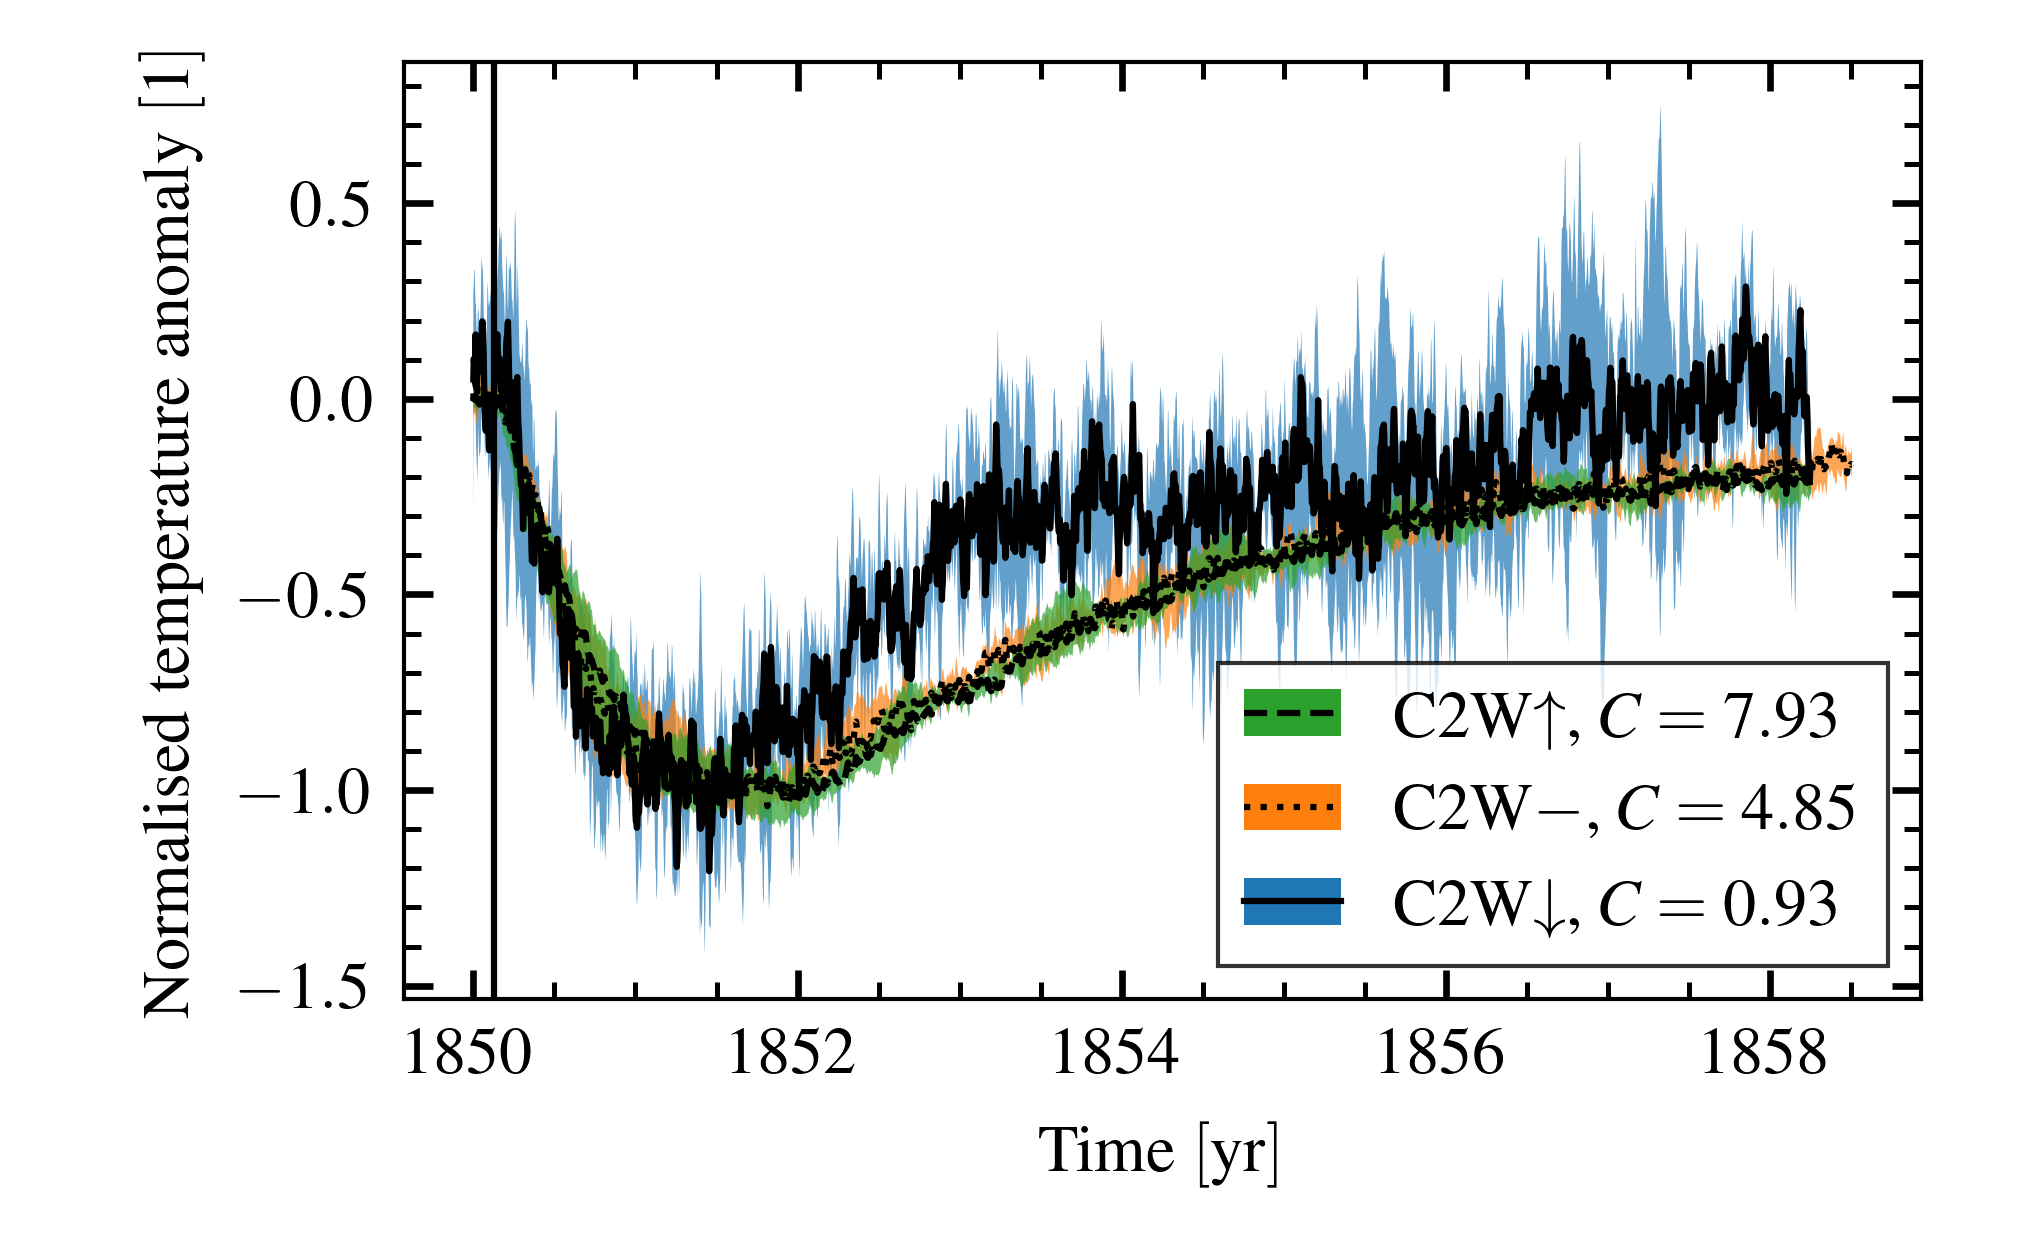
\includegraphics[width=0.95\textwidth]{figures/compare-waveform-max.png}
  \end{center}
  \caption{Normalized temperature response to three different-size volcanic eruptions,
    by setting a maximum peak value}
  \label{fig:temp_norm_max}
\end{figure}

\begin{figure}
  \begin{center}
    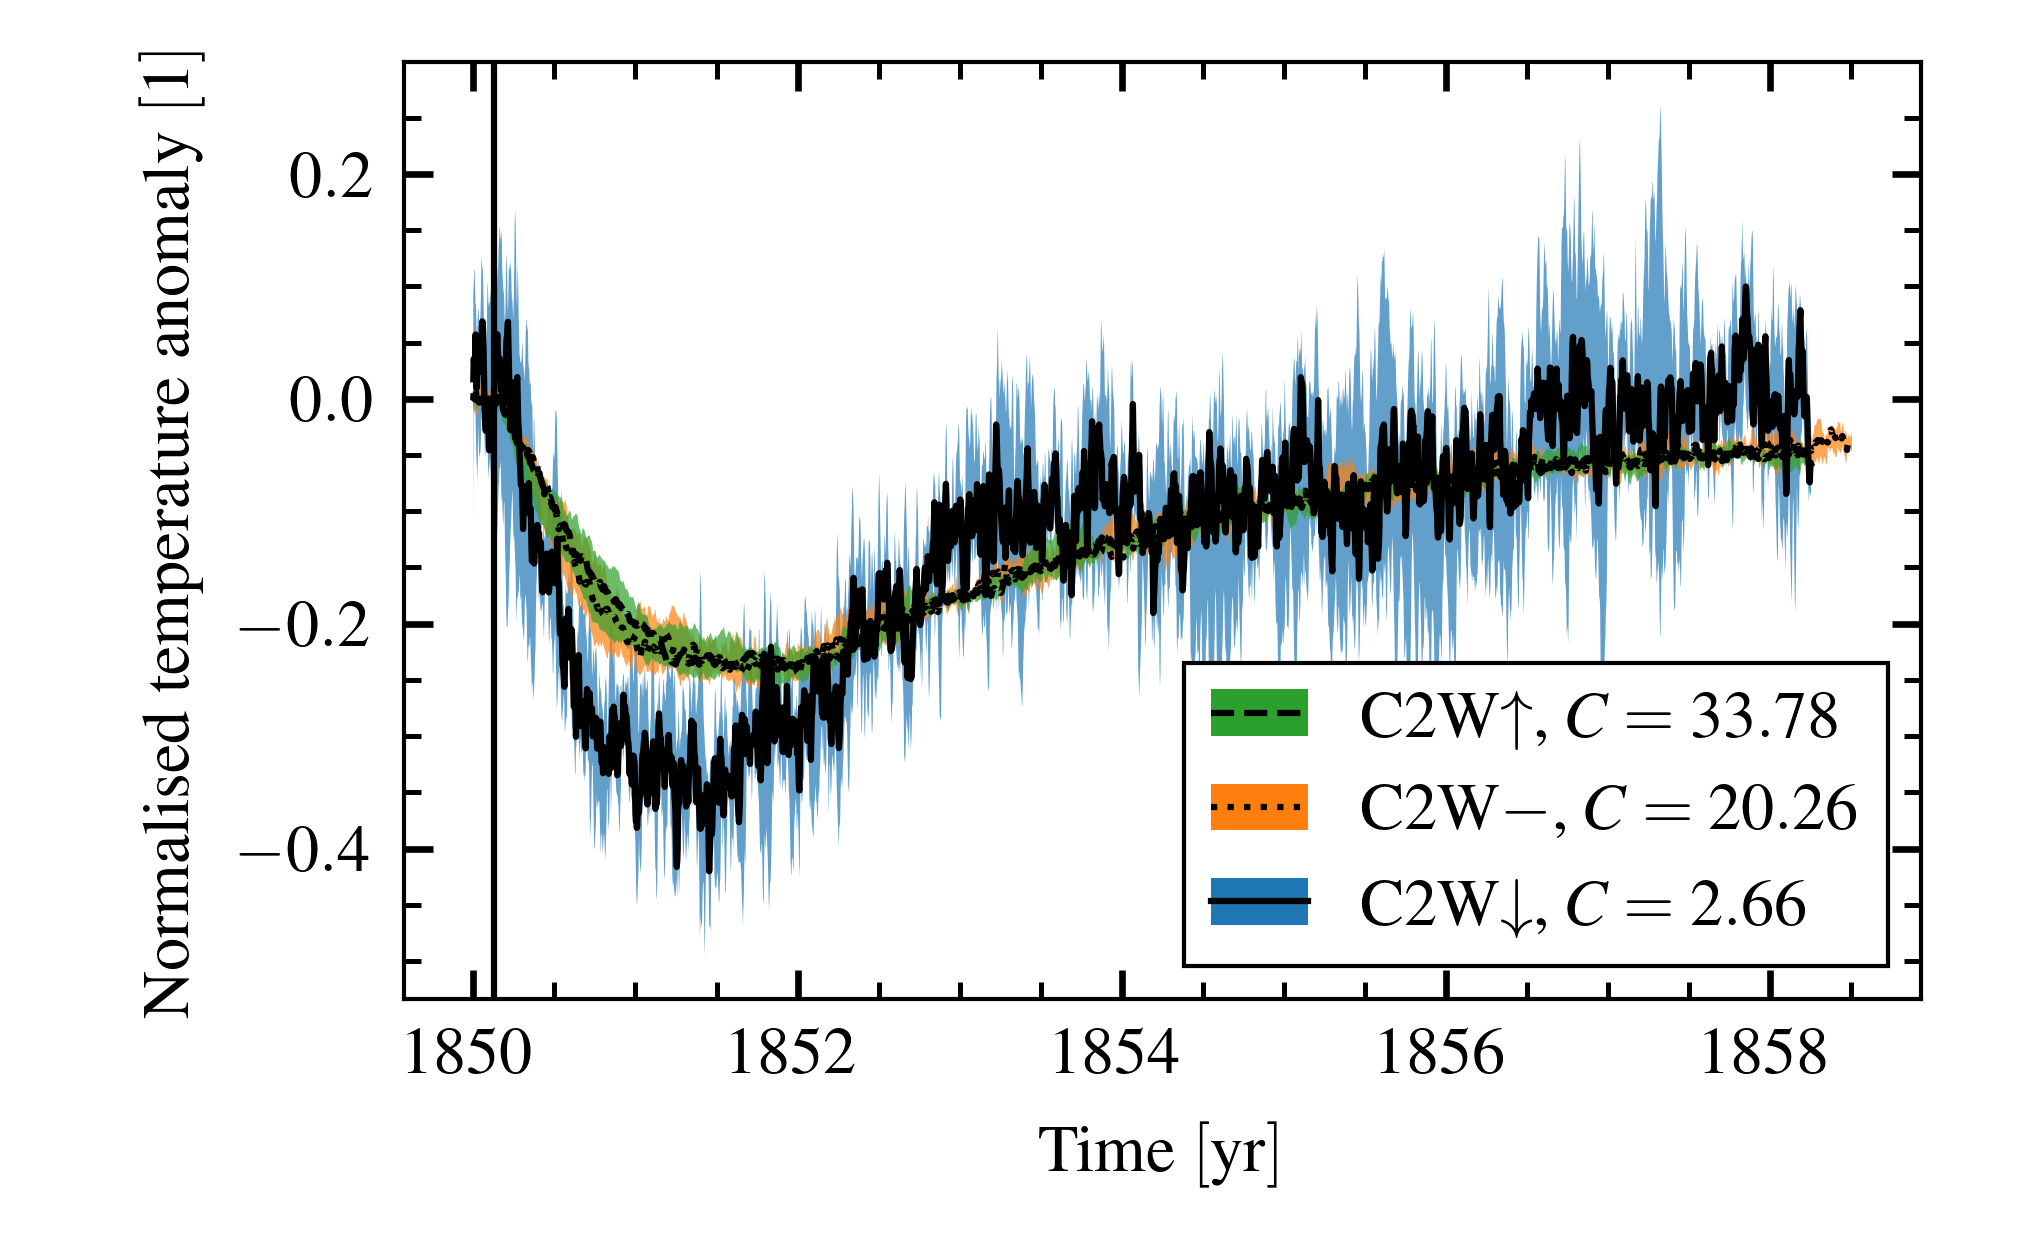
\includegraphics[width=0.95\textwidth]{figures/compare-waveform-integrate.png}
  \end{center}
  \caption{Normalized temperature response to three different-size volcanic eruptions,
    using integration, i.e., they all integrate to one}
  \label{fig:temp_norm_int}
\end{figure}

\paragraph*{Superposing volcanoes}

Let us now look at how the temperature behave when forced by two eruptions occurring
close in time (four years apart), shown in \cref{fig:double-overlap-superpose}. The
temperature is still perturbed as the second eruption happen, but when comparing this
with the superposition of the temperature time series of two single eruption events,
their alignment is quite good. Therefore, we cannot from this say that the temperature
response is sensitive to overlapping eruptions.

\begin{figure}
  \begin{center}
    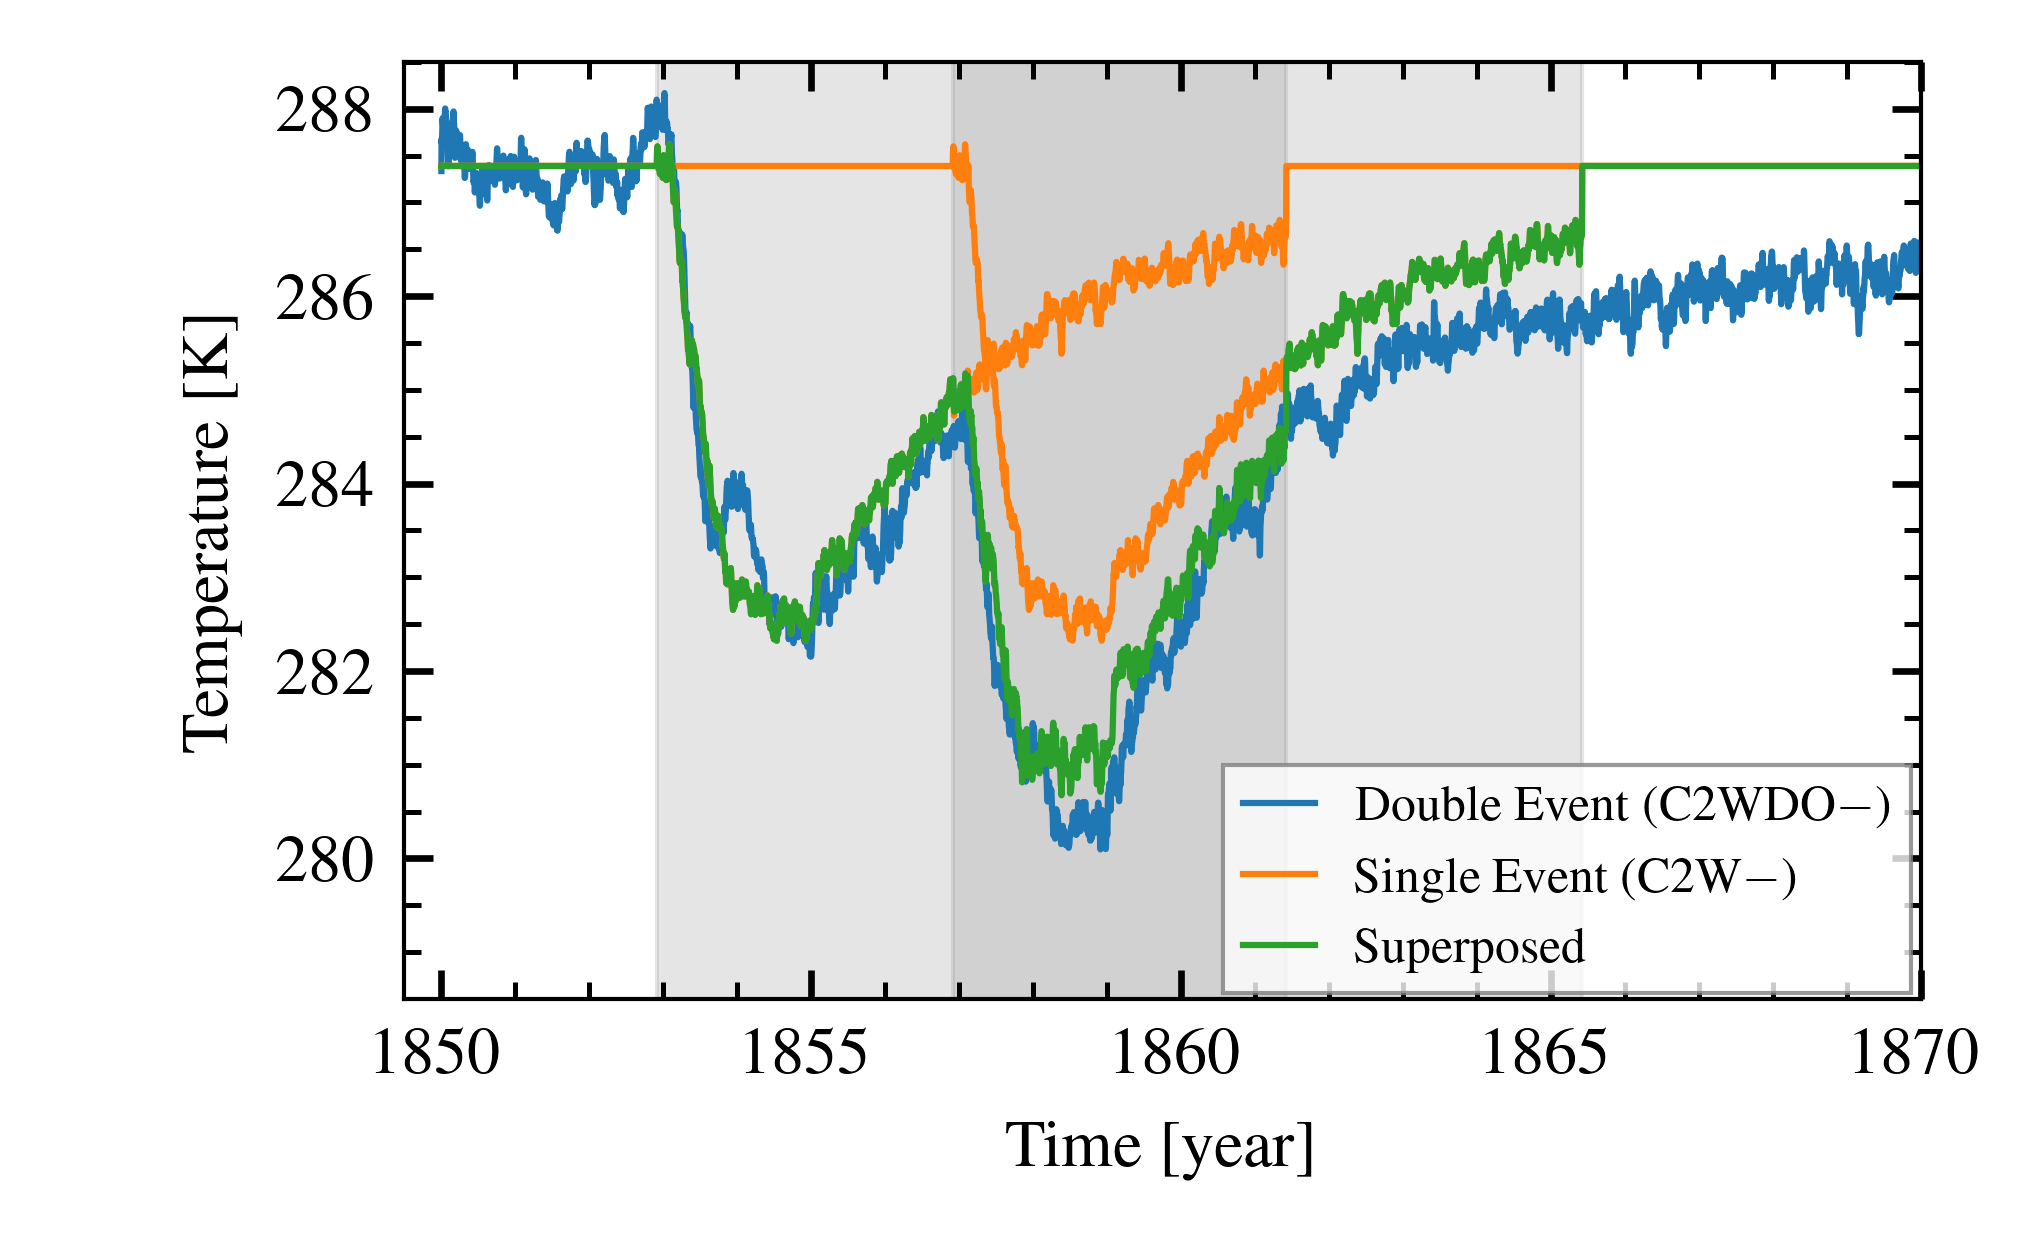
\includegraphics[width=0.95\textwidth]{figures/double-overlap-superpose.png}
  \end{center}
  \caption{Double-eruption event, where the temperature responses from the two eruptions
    overlap. That is, the second equivalent eruption occur as the temperature is still
    perturbed from the first eruption}
  \label{fig:double-overlap-superpose}
\end{figure}

\paragraph*{Parameter scan}

So far we have been focusing on temperature. We here look more closely into the
different forcings as well. This comparison is motivated by \citet{gregory2016},
specifically their figure 4 which compare annual mean aerosol optical depth with
radiative forcing. \Cref{fig:aod_vs_toa_full} show annual mean values from the three
simulation cases along with the gradient obtained by \citet{gregory2016} (\(-19\)).
First off, the \acrshort{toa} values are clearly much smaller compared the
\acrshort{aod} than what was the case for \citet{gregory2016} and the data used in their
figure.

\begin{figure}
  \begin{center}
    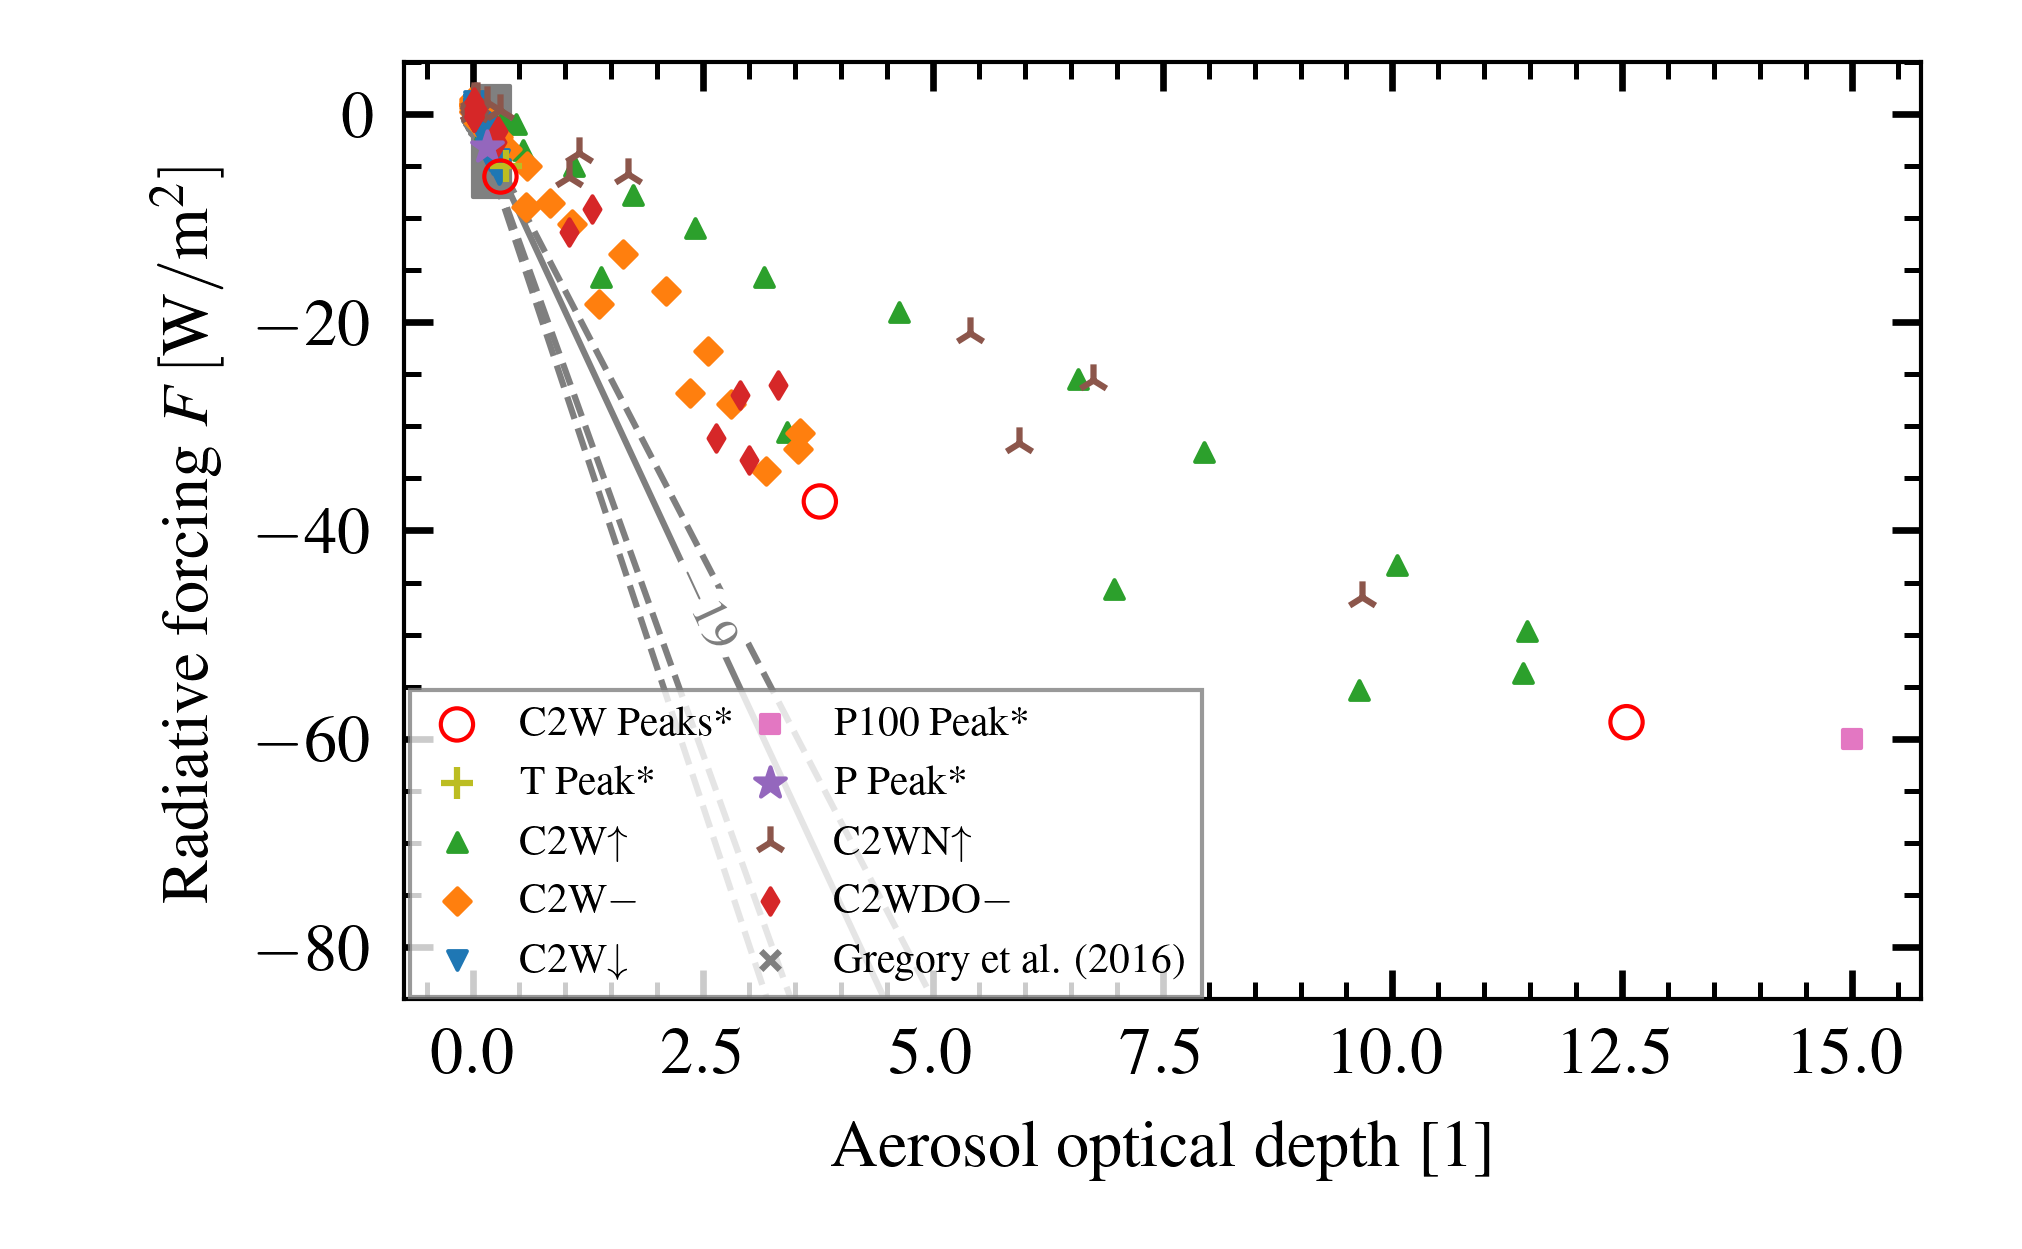
\includegraphics[width=0.95\textwidth]{figures/aod_vs_toa_avg_full.png}
  \end{center}
  \caption{\acrshort{aod} versus \acrshort{toa}, full size. Same type as \cite{gregory2016}}
  \label{fig:aod_vs_toa_full}
\end{figure}

\begin{figure}
  \begin{center}
    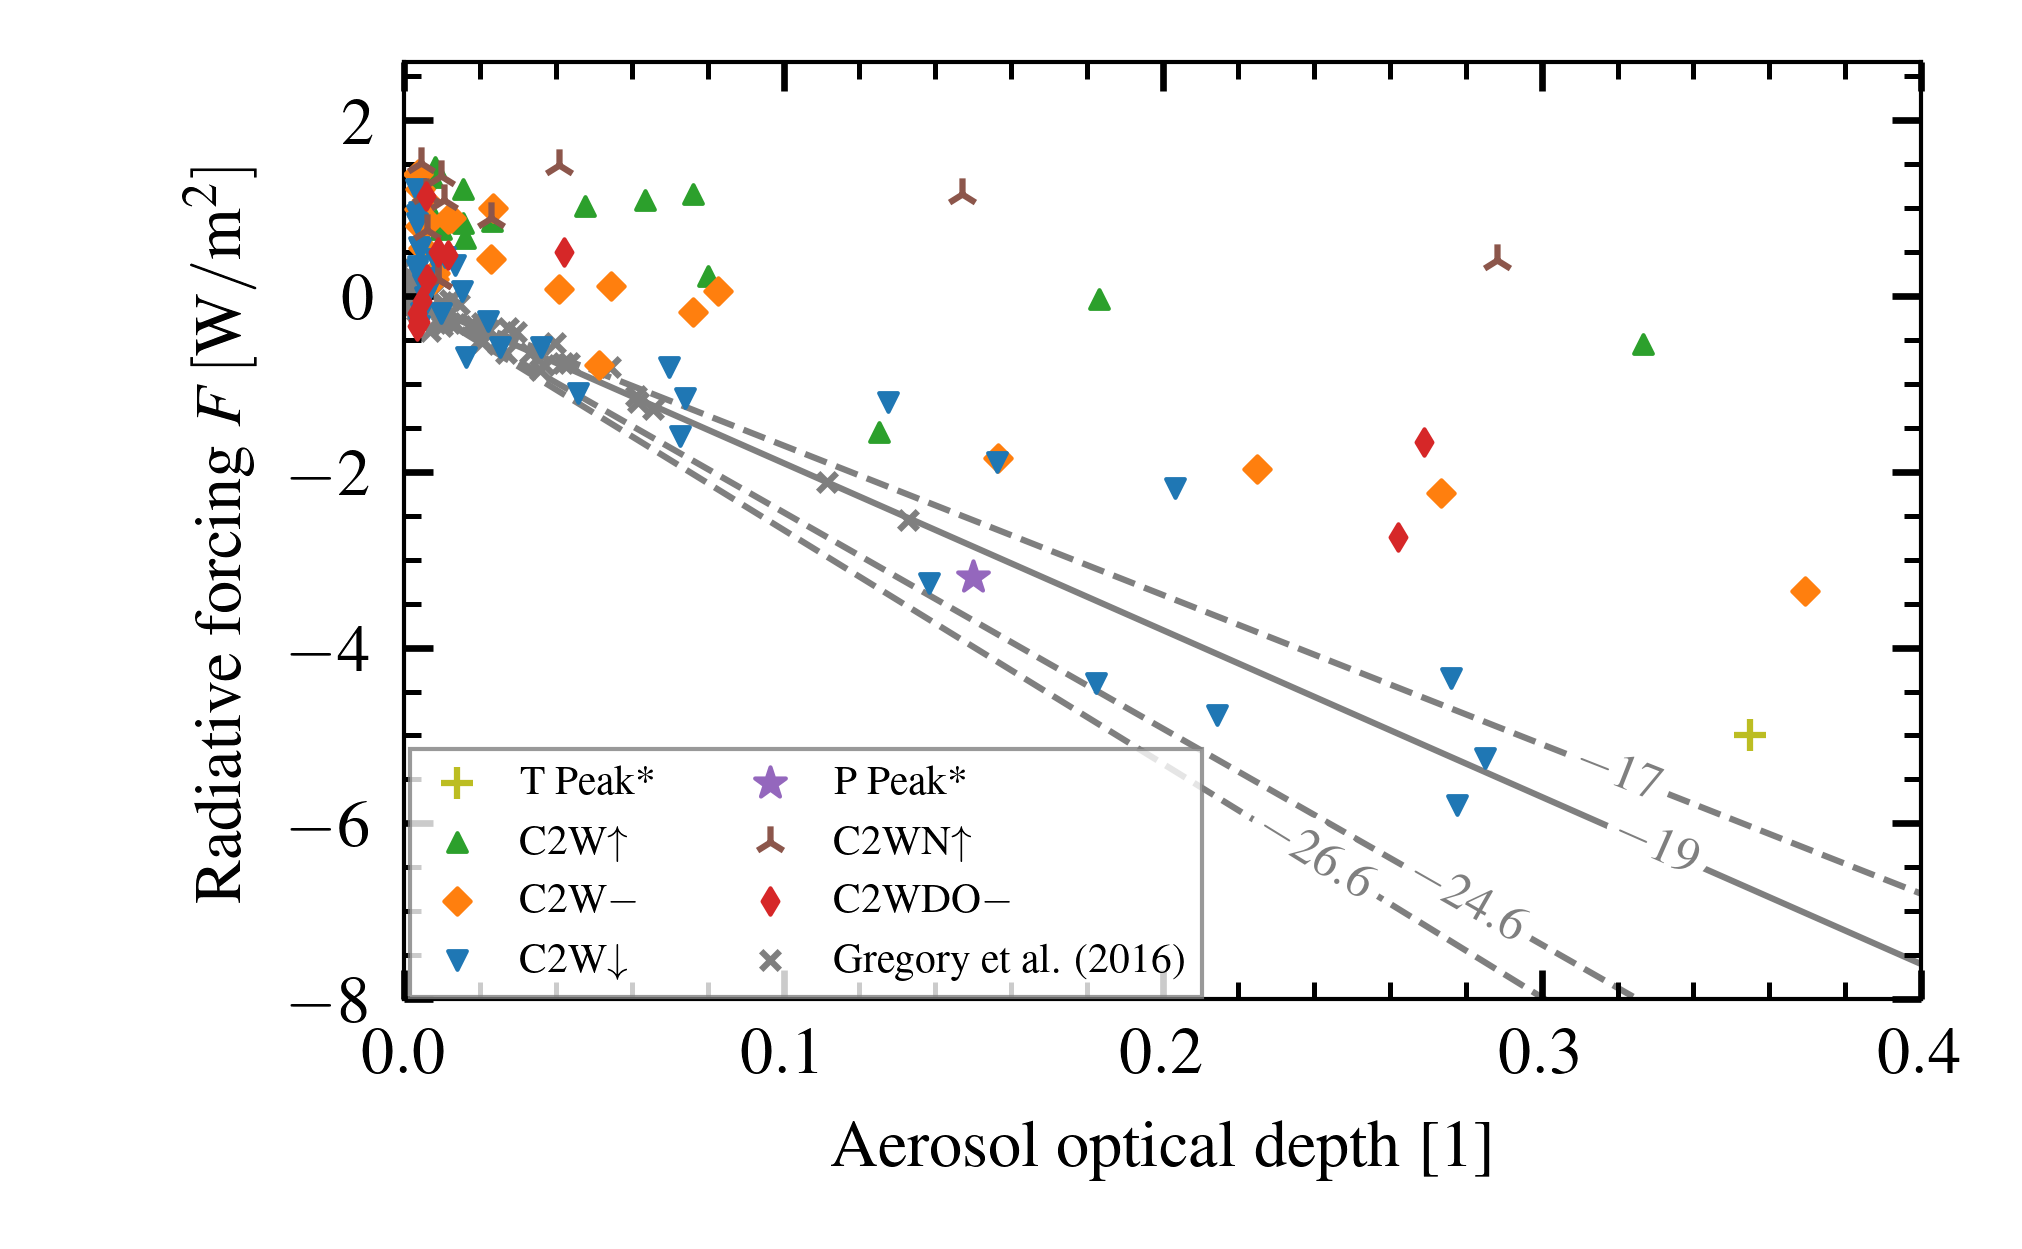
\includegraphics[width=0.95\textwidth]{figures/aod_vs_toa_avg_inset.png}
  \end{center}
  \caption{\acrshort{aod} versus \acrshort{toa}, inset. Same type as \cite{gregory2016}}
  \label{fig:aod_vs_toa_inset}
\end{figure}

\begin{figure}
  \begin{center}
    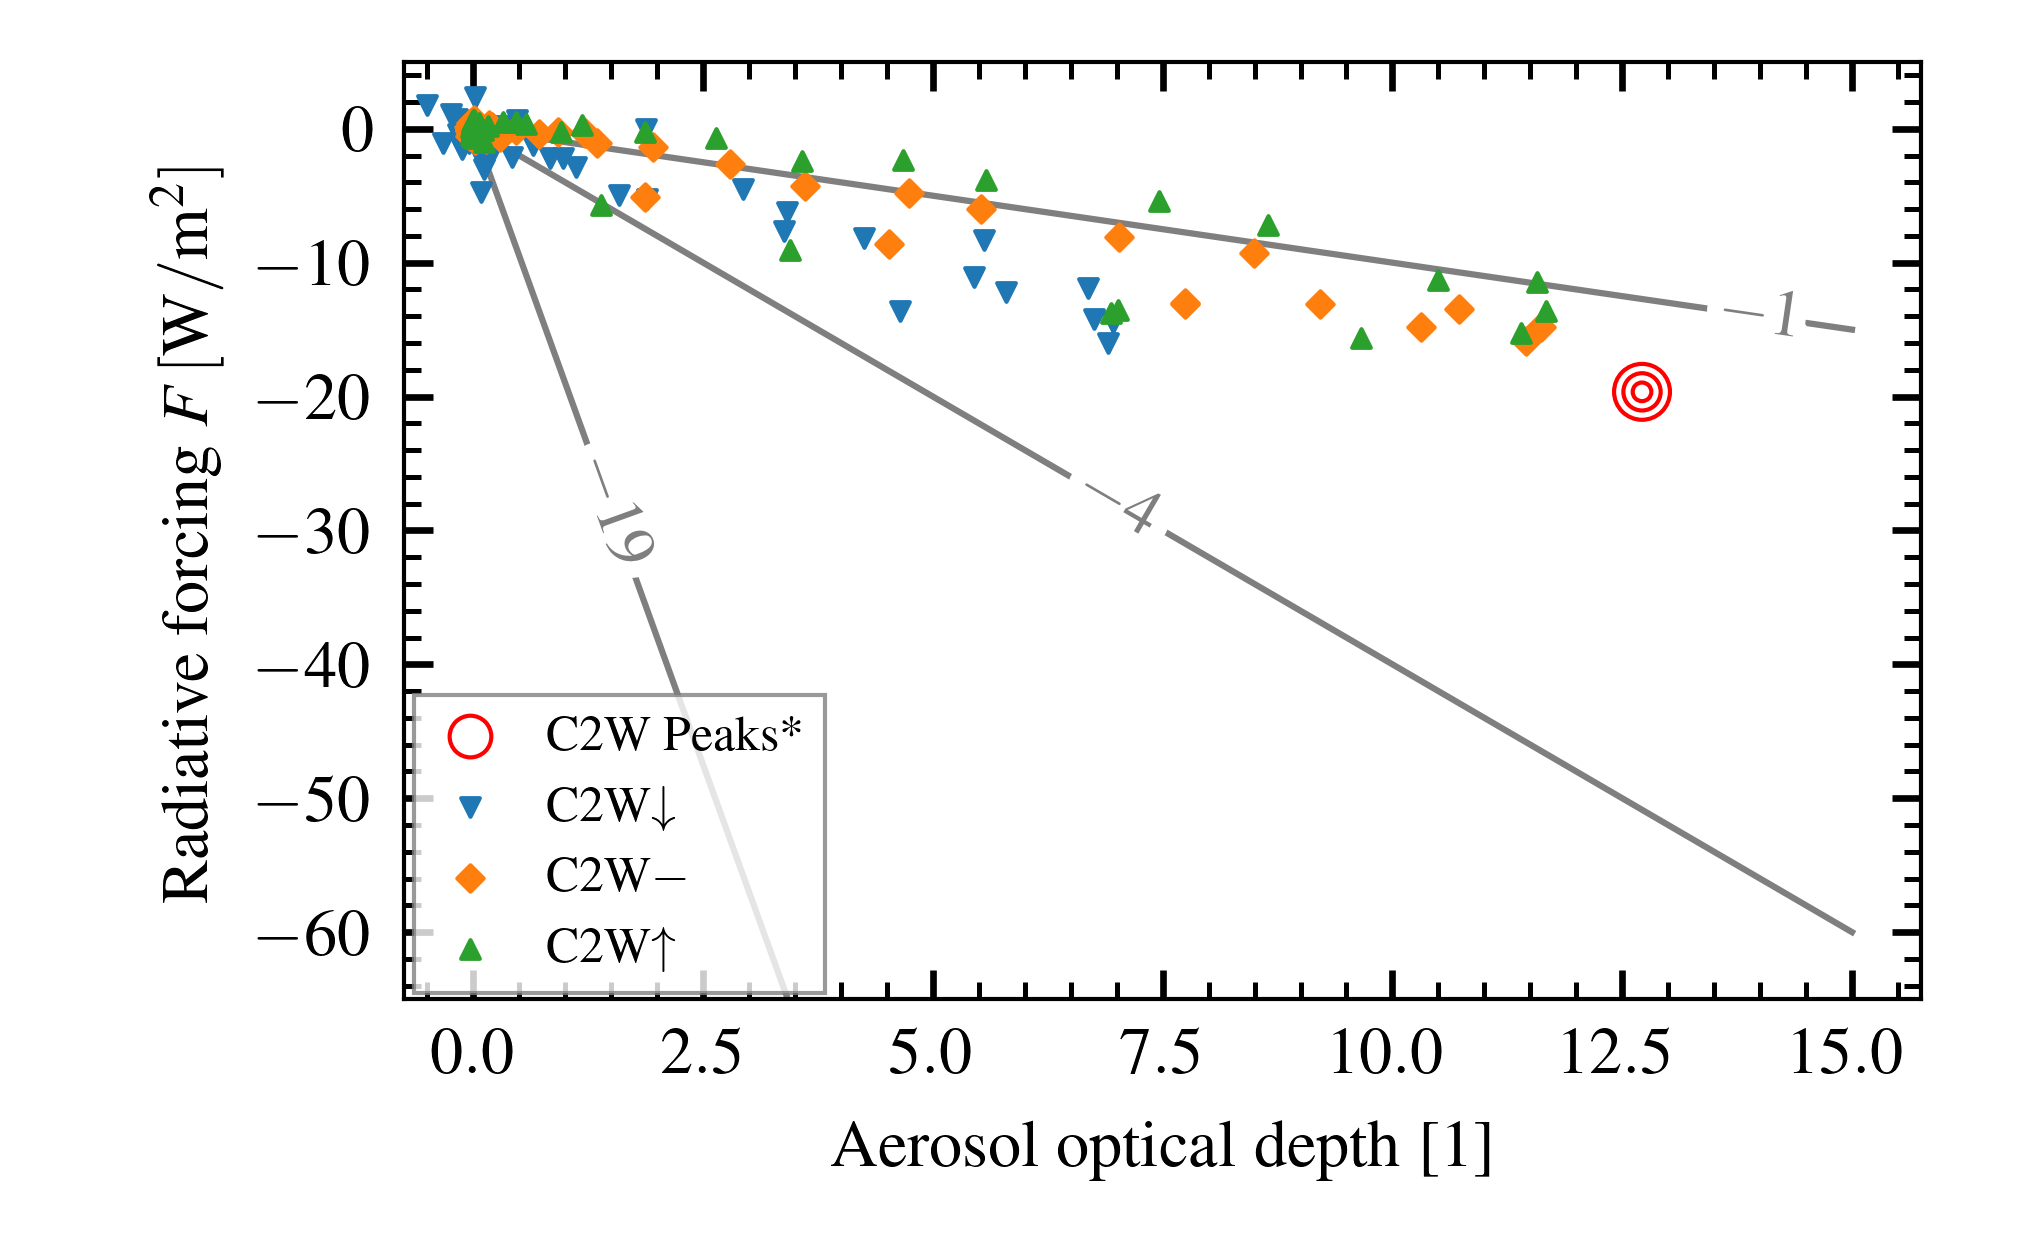
\includegraphics[width=0.95\textwidth]{figures/aod_vs_toa_avg_scaled.png}
  \end{center}
  \caption{
    \acrshort{aod} versus \acrshort{toa}, scaled so the peak values of the different
    volcano magnitudes are aligned. Same type as \cite{gregory2016}
  }
  \label{fig:aod_vs_toa_scaled}
\end{figure}

\begin{figure}
  \begin{center}
    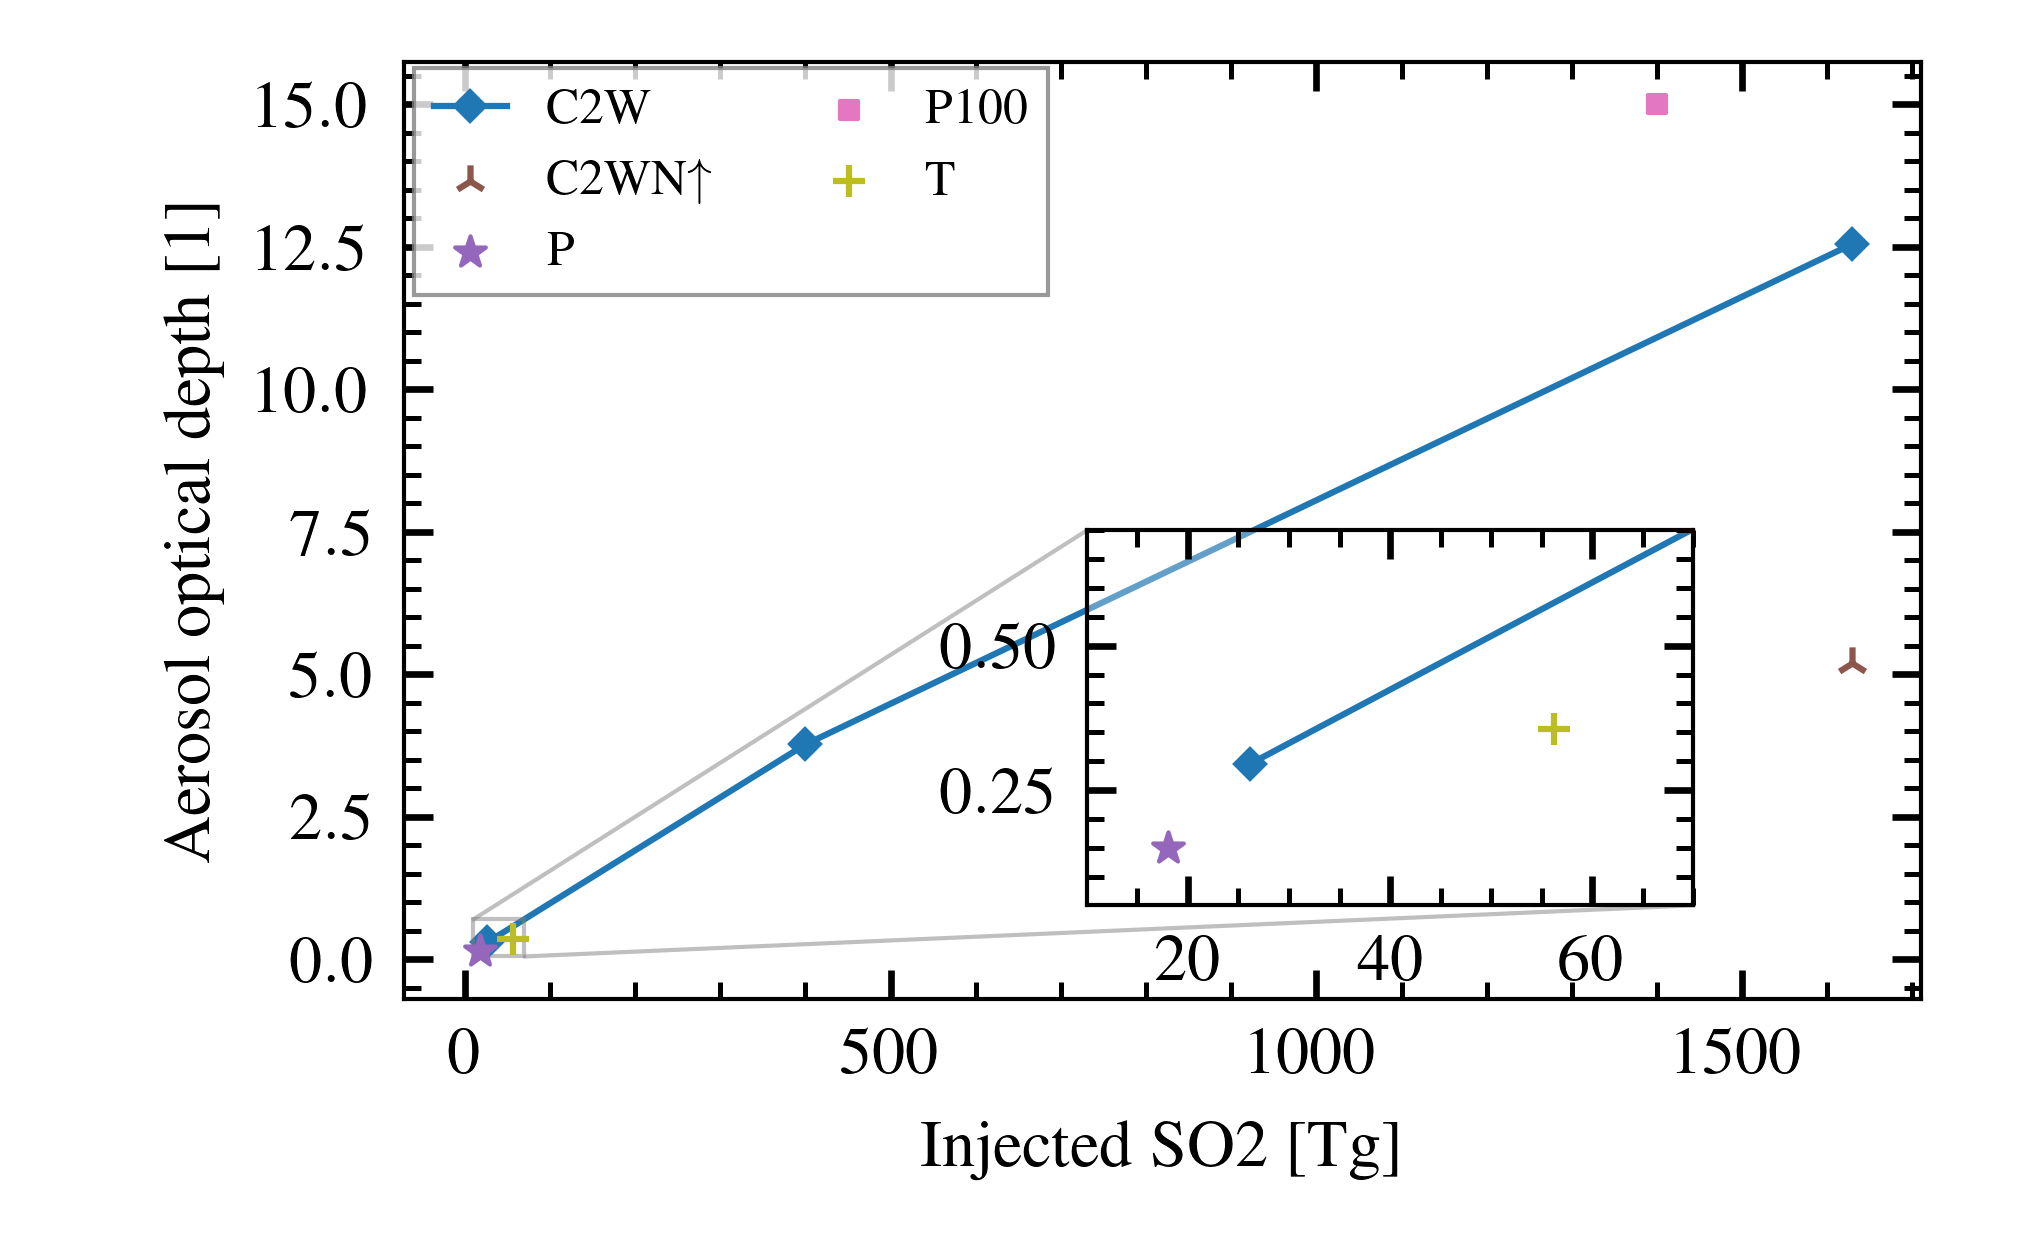
\includegraphics[width=0.95\textwidth]{figures/injection_vs_aod.png}
  \end{center}
  \caption{Injected \ce{SO2} versus \acrshort{aod}}
  \label{fig:so2_vs_aod}
\end{figure}

\begin{figure}
  \begin{center}
    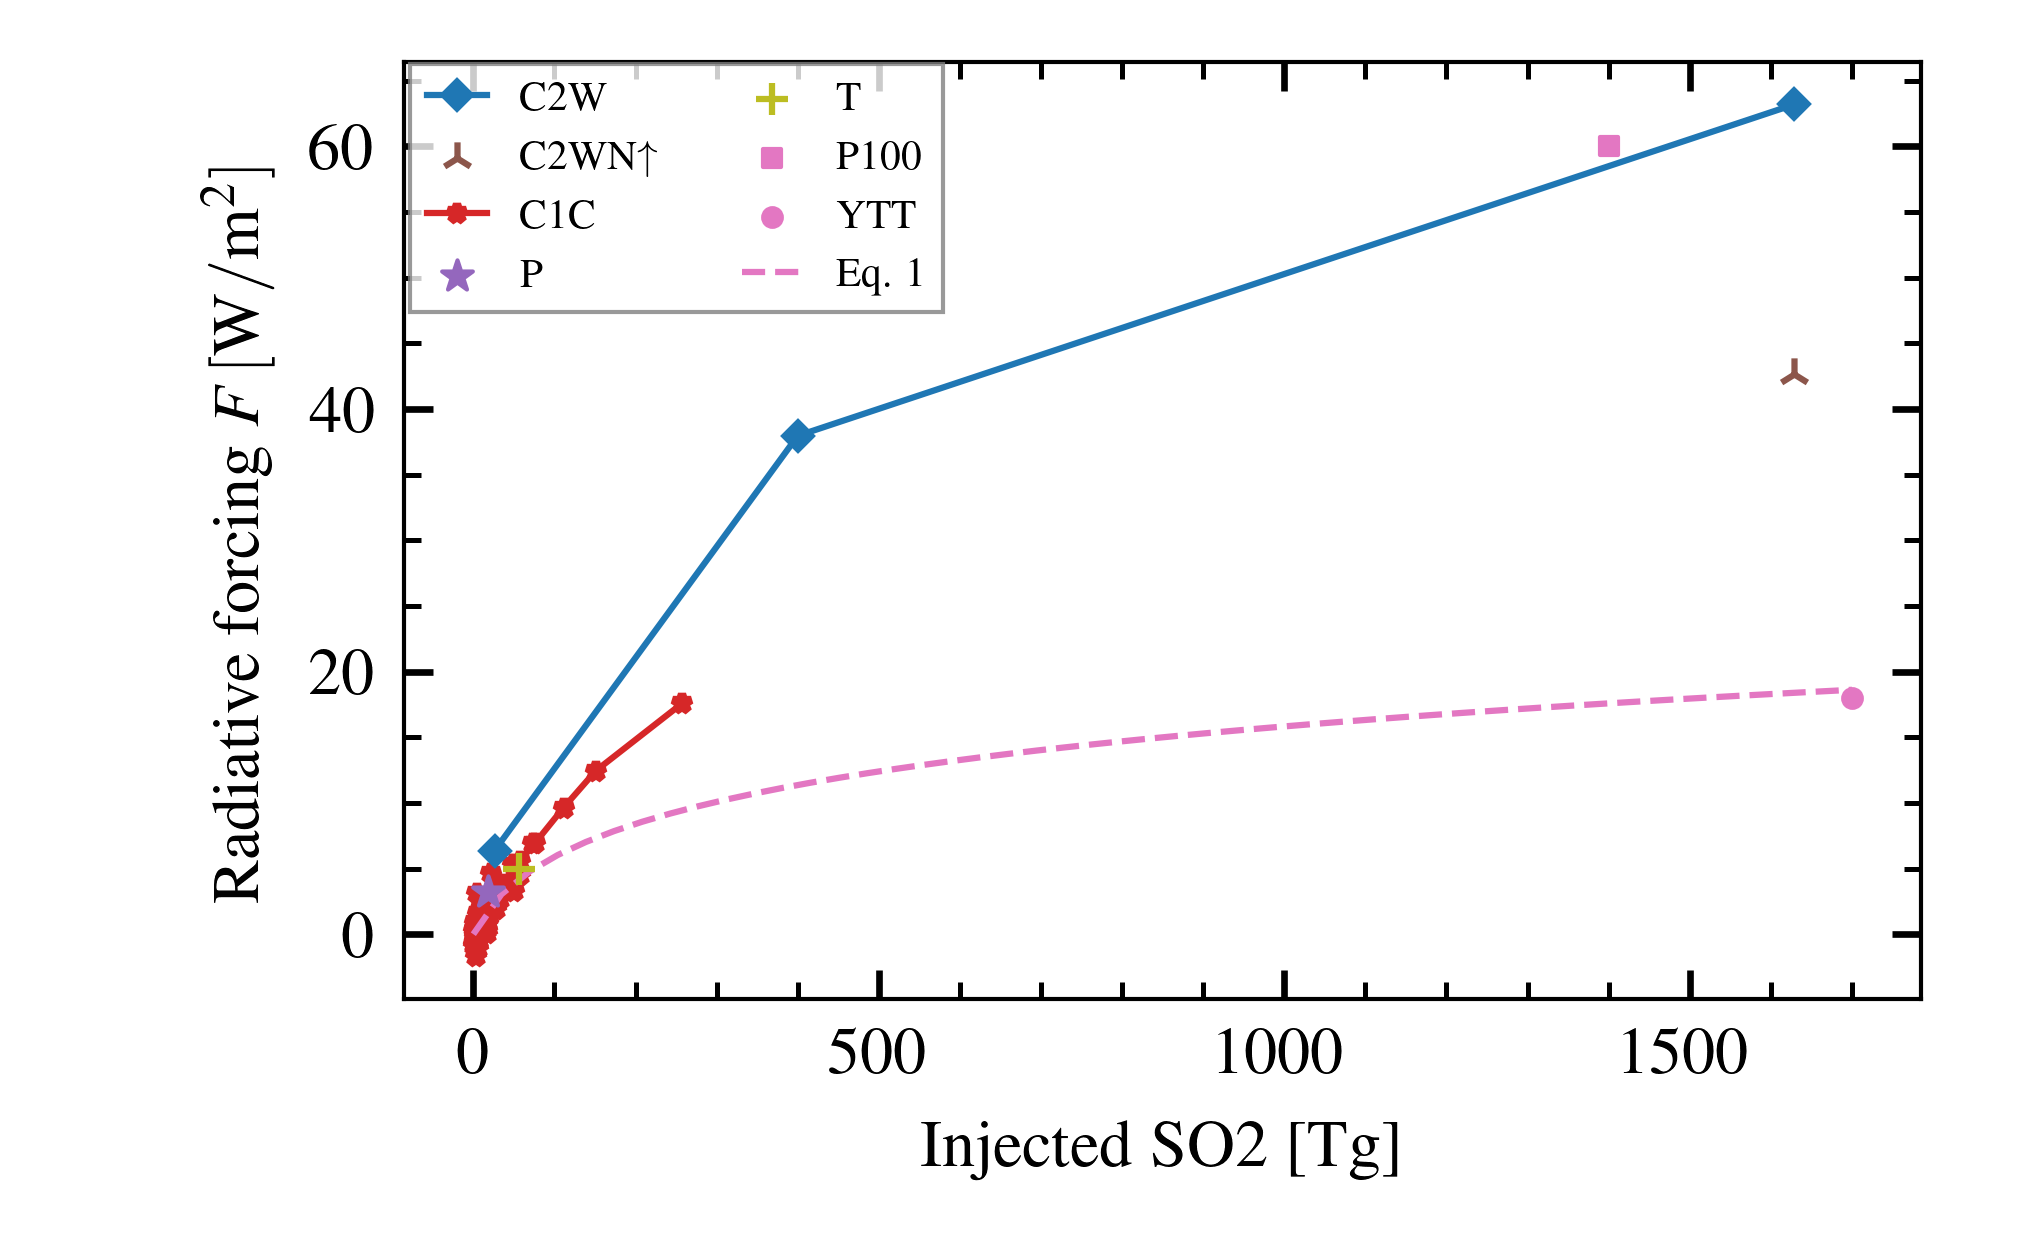
\includegraphics[width=0.95\textwidth]{figures/injection_vs_toa.png}
  \end{center}
  \caption{Injected \ce{SO2} versus \acrshort{toa} radiative imbalance}
  \label{fig:so2_vs_toa}
\end{figure}

\begin{figure}
  \begin{center}
    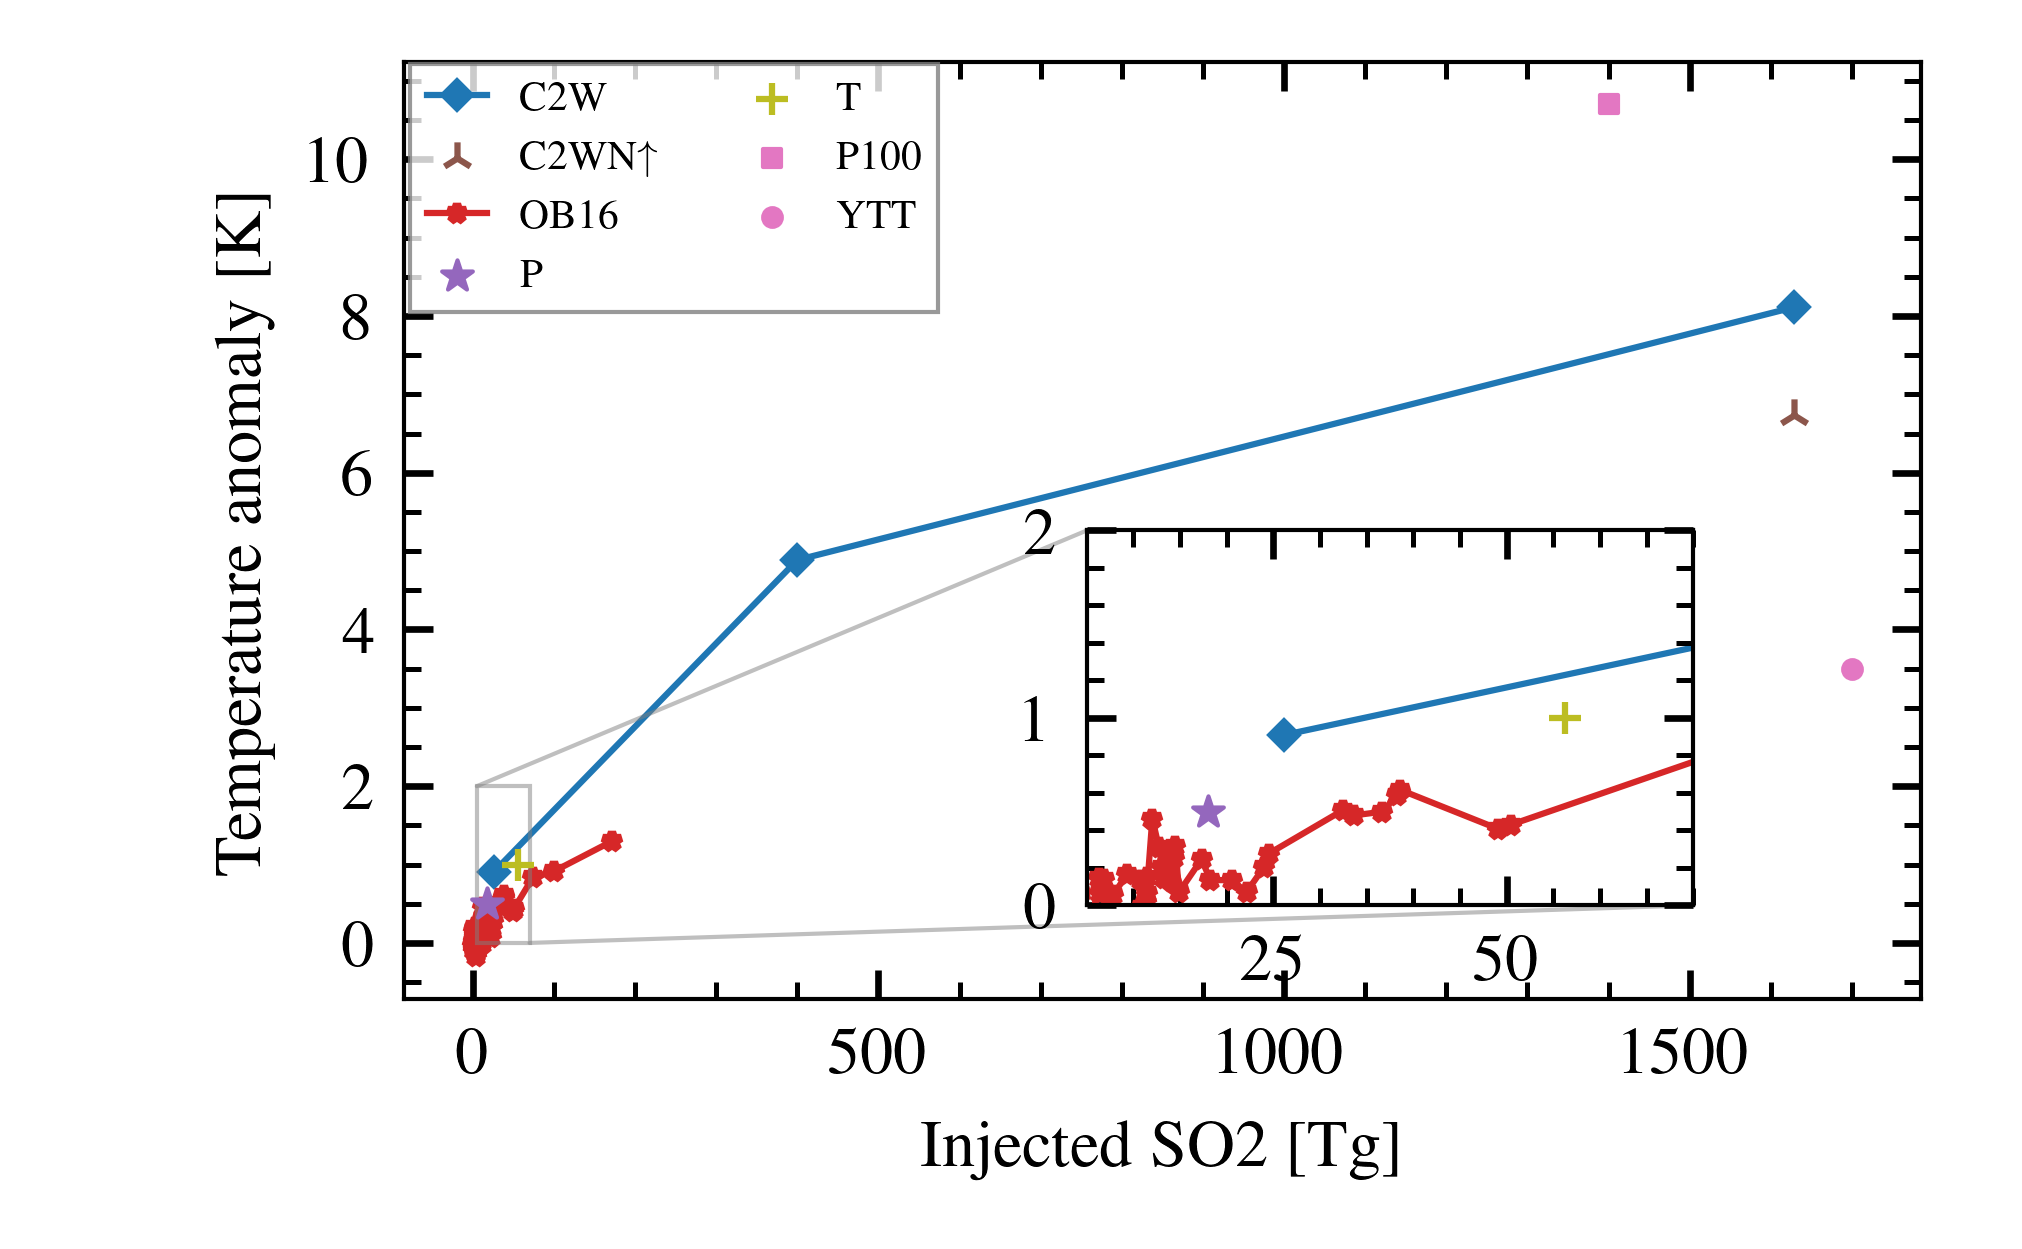
\includegraphics[width=0.95\textwidth]{figures/injection_vs_temperature.png}
  \end{center}
  \caption{Injected \ce{SO2} versus temperature}
  \label{fig:so2_vs_temp}
\end{figure}

\begin{figure}
  \begin{center}
    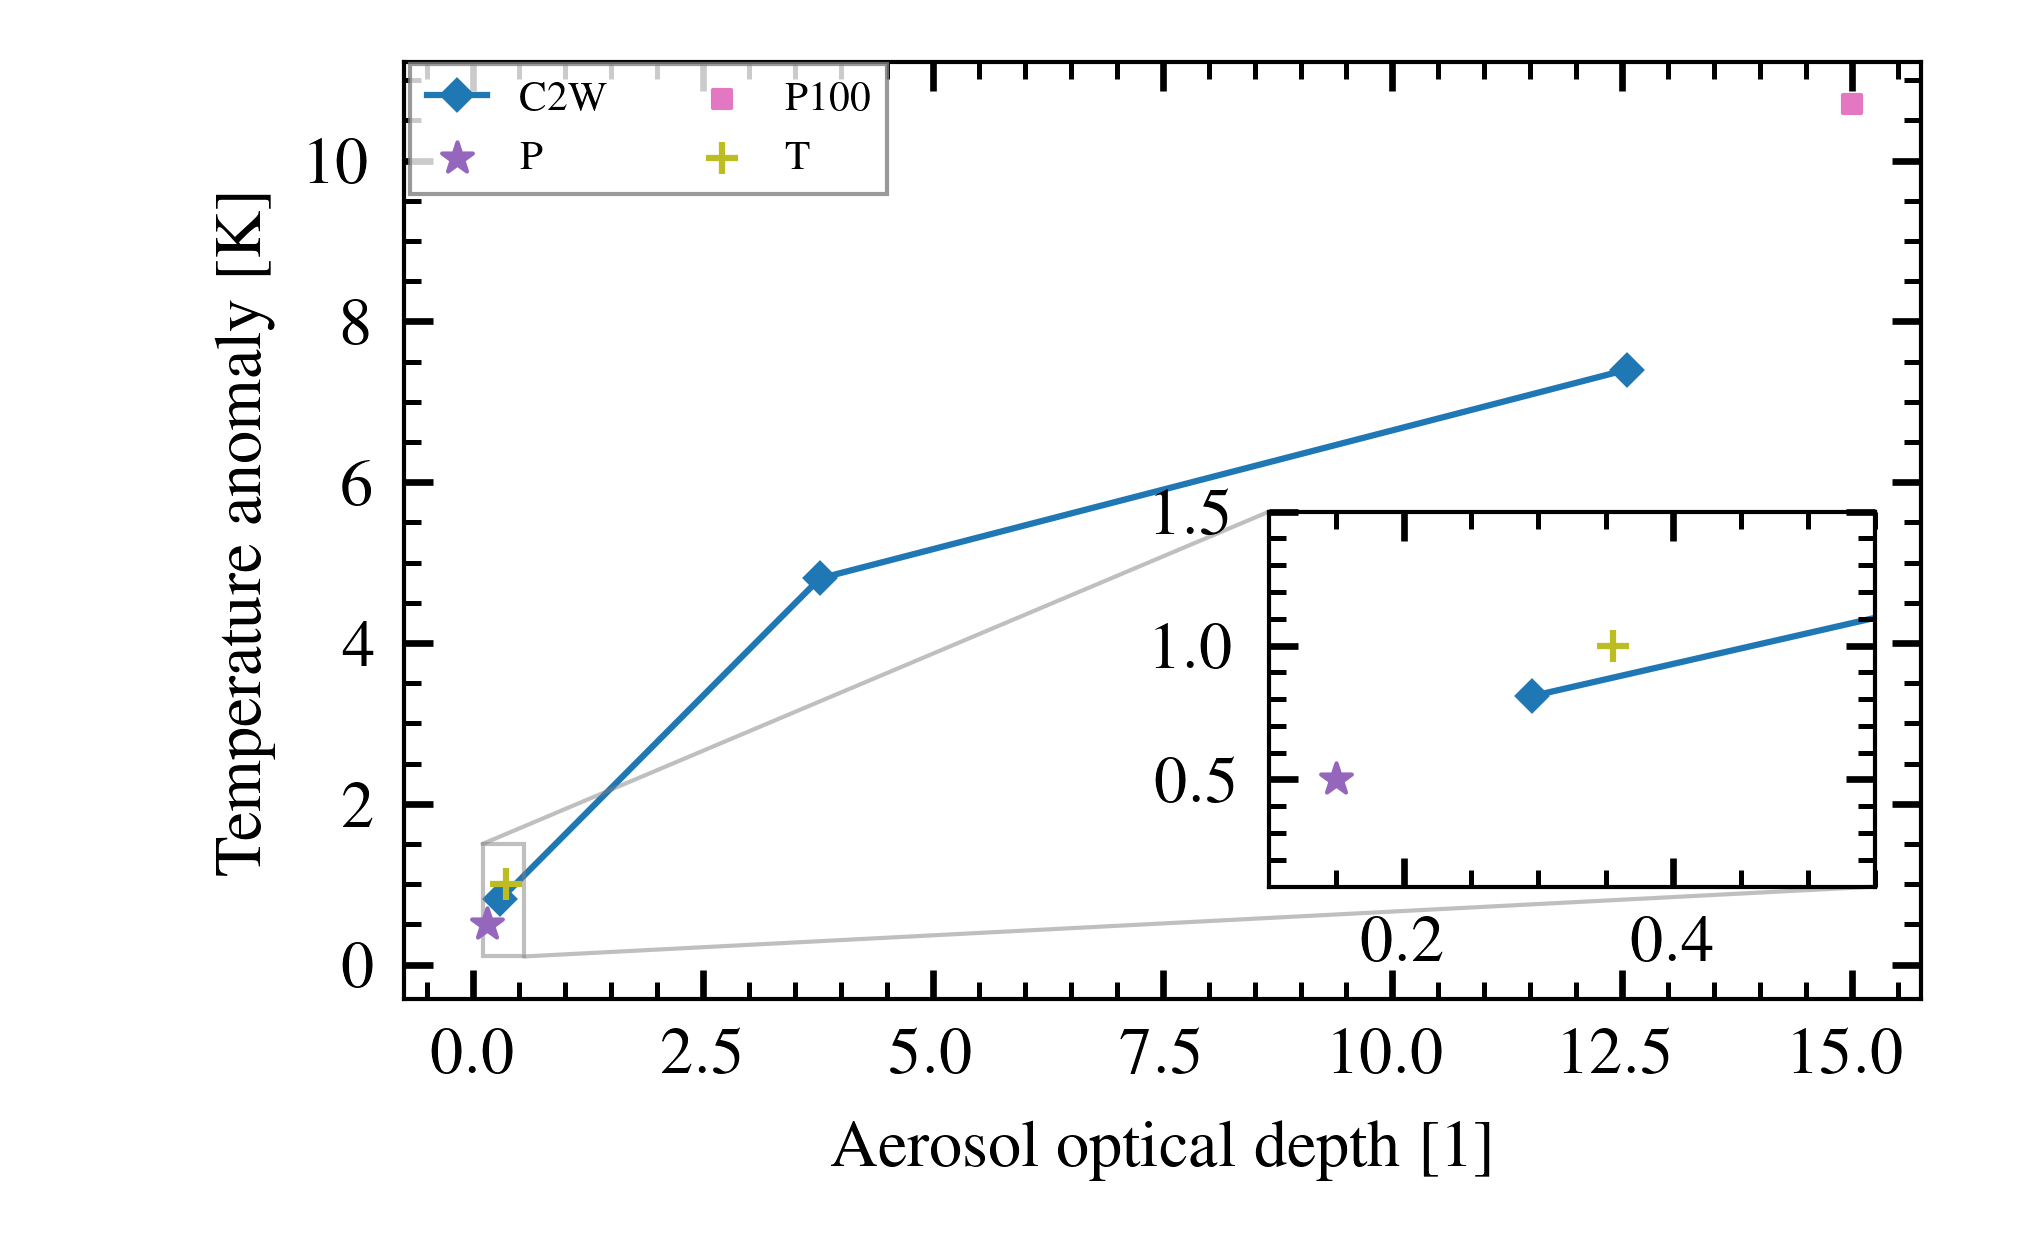
\includegraphics[width=0.95\textwidth]{figures/aod_vs_temperature.png}
  \end{center}
  \caption{\acrshort{aod} versus temperature}
  \label{fig:aod_vs_temp}
\end{figure}

\begin{figure}
  \begin{center}
    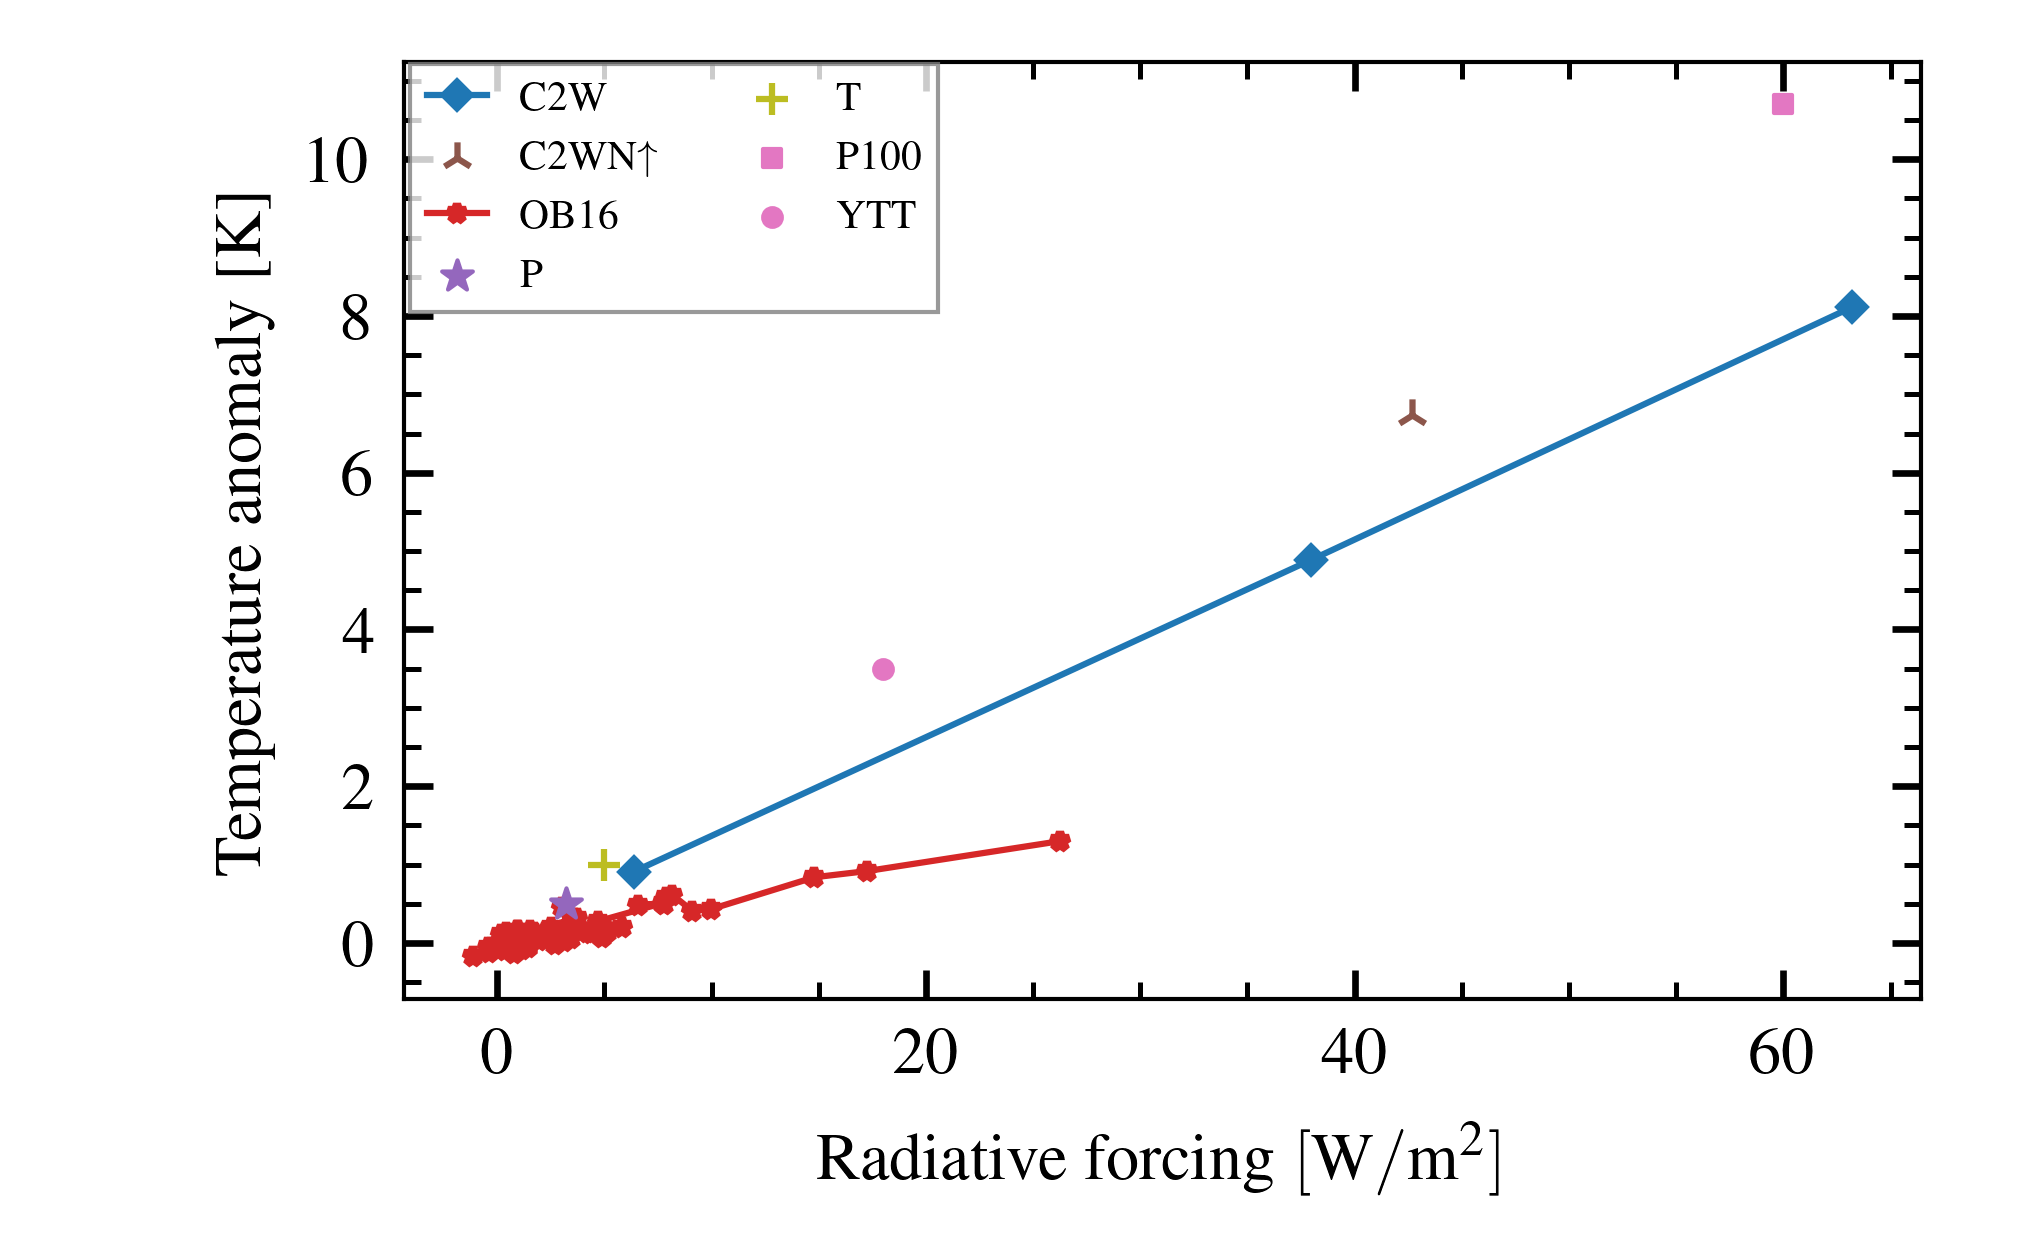
\includegraphics[width=0.95\textwidth]{figures/toa_vs_temperature.png}
  \end{center}
  \caption{\acrshort{toa} versus temperature}
  \label{fig:toa_vs_temp}
\end{figure}

\clearpage

% %%%%%%%%%%%%%%%%%%%%%%%%%%%%%%%%%%%%%%%%%%%%%%%%%%%%%%%%%%%%%%%%%%%%%%%%%%%%%%%%%%%%%%
% ACKNOWLEDGMENTS
% %%%%%%%%%%%%%%%%%%%%%%%%%%%%%%%%%%%%%%%%%%%%%%%%%%%%%%%%%%%%%%%%%%%%%%%%%%%%%%%%%%%%%%
% \acknowledgments

% Keep acknowledgments (note correct spelling: no ``e'' between the ``g'' and ``m'') as
% brief as possible. In general, acknowledge only direct help in writing or research.
% Financial support (e.g., grant numbers) for the work done, for an author, or for the
% laboratory where the work was performed is best acknowledged here rather than as
% footnotes to the title or to an author's name. Contribution numbers (if the work has
% been published by the author's institution or organization) should be included as
% footnotes on the title page, not in the acknowledgments.

% %%%%%%%%%%%%%%%%%%%%%%%%%%%%%%%%%%%%%%%%%%%%%%%%%%%%%%%%%%%%%%%%%%%%%%%%%%%%%%%%%%%%%%
% DATA AVAILABILITY STATEMENT
% %%%%%%%%%%%%%%%%%%%%%%%%%%%%%%%%%%%%%%%%%%%%%%%%%%%%%%%%%%%%%%%%%%%%%%%%%%%%%%%%%%%%%%
% \datastatement

% The data availability statement is where authors should describe how the data
% underlying the findings within the article can be accessed and reused. Authors should
% attempt to provide unrestricted access to all data and materials underlying reported
% findings. If data access is restricted, authors must mention this in the statement.

% %%%%%%%%%%%%%%%%%%%%%%%%%%%%%%%%%%%%%%%%%%%%%%%%%%%%%%%%%%%%%%%%%%%%%%%%%%%%%%%%%%%%%%
% APPENDIXES
% %%%%%%%%%%%%%%%%%%%%%%%%%%%%%%%%%%%%%%%%%%%%%%%%%%%%%%%%%%%%%%%%%%%%%%%%%%%%%%%%%%%%%%
%
% Use \appendix if there is only one appendix.
% \appendix

% Use \appendix[A], \appendix[B], if you have multiple appendixes.
% \appendix[A]

% Appendix title is necessary! For appendix title:
% \appendixtitle{}

% Appendix section numbering (note, skip \section and begin with \subsection)
% \subsection{First primary heading}

% \subsubsection{First secondary heading}

% \paragraph{First tertiary heading}

% Important!
% \appendcaption{<appendix letter and number>}{<caption>}
% must be used for figures and tables in appendixes, e.g.,
%
% \begin{figure}
% \noindent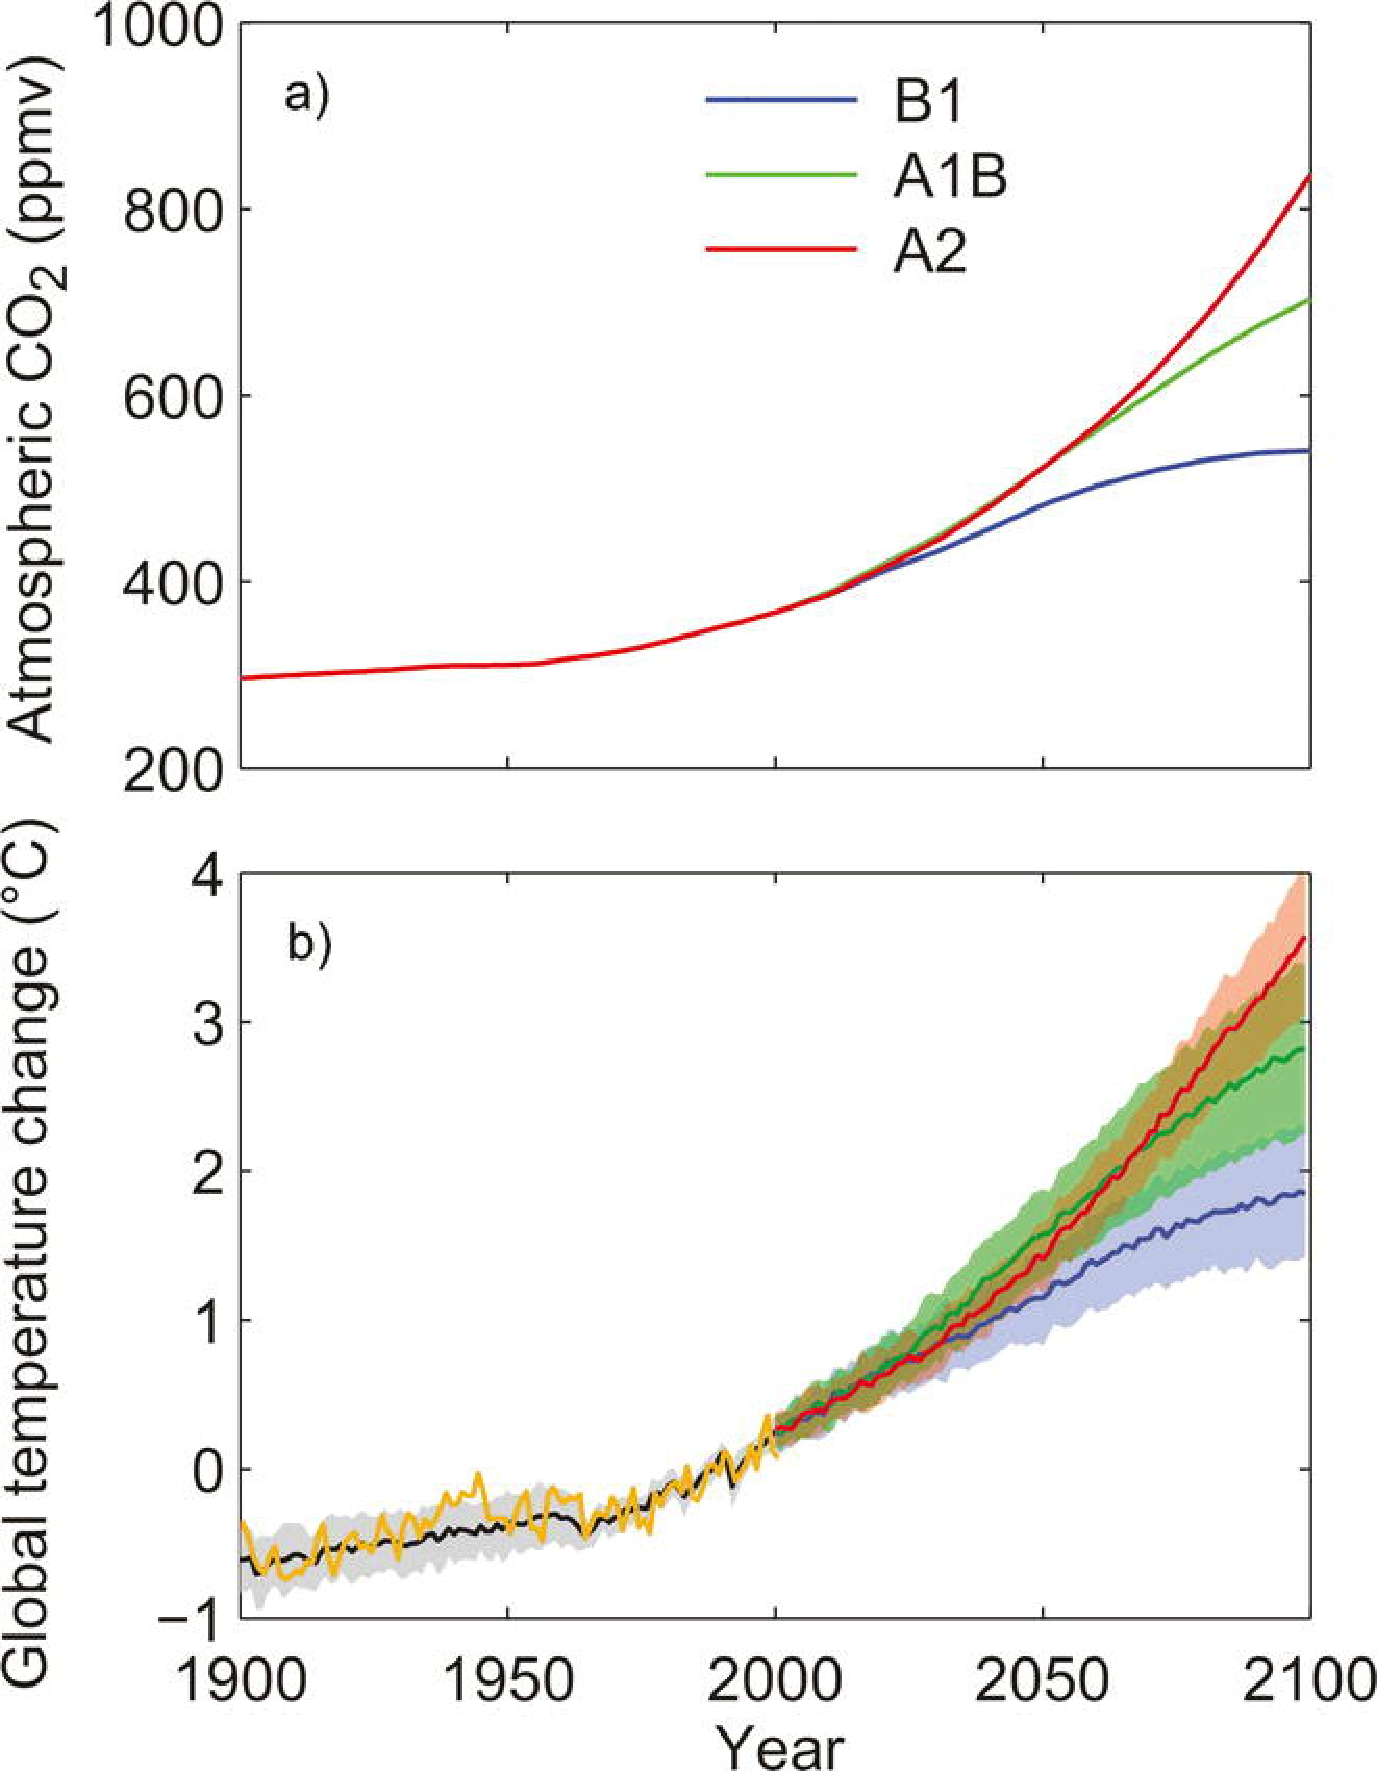
\includegraphics[width=19pc,angle=0]{figure01.pdf}\\
% \appendcaption{A1}{Caption here.}
% \end{figure}
%
% All appendix figures/tables should be placed in order AFTER the main figures/tables,
% i.e., tables, appendix tables, figures, appendix figures.
%
% %%%%%%%%%%%%%%%%%%%%%%%%%%%%%%%%%%%%%%%%%%%%%%%%%%%%%%%%%%%%%%%%%%%%%%%%%%%%%%%%%%%%%%
% REFERENCES
% %%%%%%%%%%%%%%%%%%%%%%%%%%%%%%%%%%%%%%%%%%%%%%%%%%%%%%%%%%%%%%%%%%%%%%%%%%%%%%%%%%%%%%
% Make your BibTeX bibliography by using these commands:
\bibliographystyle{ametsoc2014}
\bibliography{references}
\clearpage
\printglossary[type=\acronymtype,title=List of Acronyms]
% %%%%%%%%%%%%%%%%%%%%%%%%%%%%%%%%%%%%%%%%%%%%%%%%%%%%%%%%%%%%%%%%%%%%%%%%%%%%%%%%%%%%%%
% TABLES
% %%%%%%%%%%%%%%%%%%%%%%%%%%%%%%%%%%%%%%%%%%%%%%%%%%%%%%%%%%%%%%%%%%%%%%%%%%%%%%%%%%%%%%
% Enter tables at the end of the document, before figures.
%
% \begin{table}[t]
%   \caption{This is a sample table caption and table layout.  Enter as many tables as
%     necessary at the end of your manuscript. Table from Lorenz (1963).}\label{t1}
%   \begin{center}
%     \begin{tabular}{ccccrrcrc}
%       \hline\hline
%       $N$  & $X$  & $Y$  & $Z$  \\
%       \hline
%       0000 & 0000 & 0010 & 0000 \\
%       0005 & 0004 & 0012 & 0000 \\
%       0010 & 0009 & 0020 & 0000 \\
%       0015 & 0016 & 0036 & 0002 \\
%       0020 & 0030 & 0066 & 0007 \\
%       0025 & 0054 & 0115 & 0024 \\
%       \hline
%     \end{tabular}
%   \end{center}
% \end{table}

% %%%%%%%%%%%%%%%%%%%%%%%%%%%%%%%%%%%%%%%%%%%%%%%%%%%%%%%%%%%%%%%%%%%%%%%%%%%%%%%%%%%%%%
% FIGURES
% %%%%%%%%%%%%%%%%%%%%%%%%%%%%%%%%%%%%%%%%%%%%%%%%%%%%%%%%%%%%%%%%%%%%%%%%%%%%%%%%%%%%%%
% Enter figures at the end of the document, after tables.
%
% \begin{figure}[t]
%   \noindent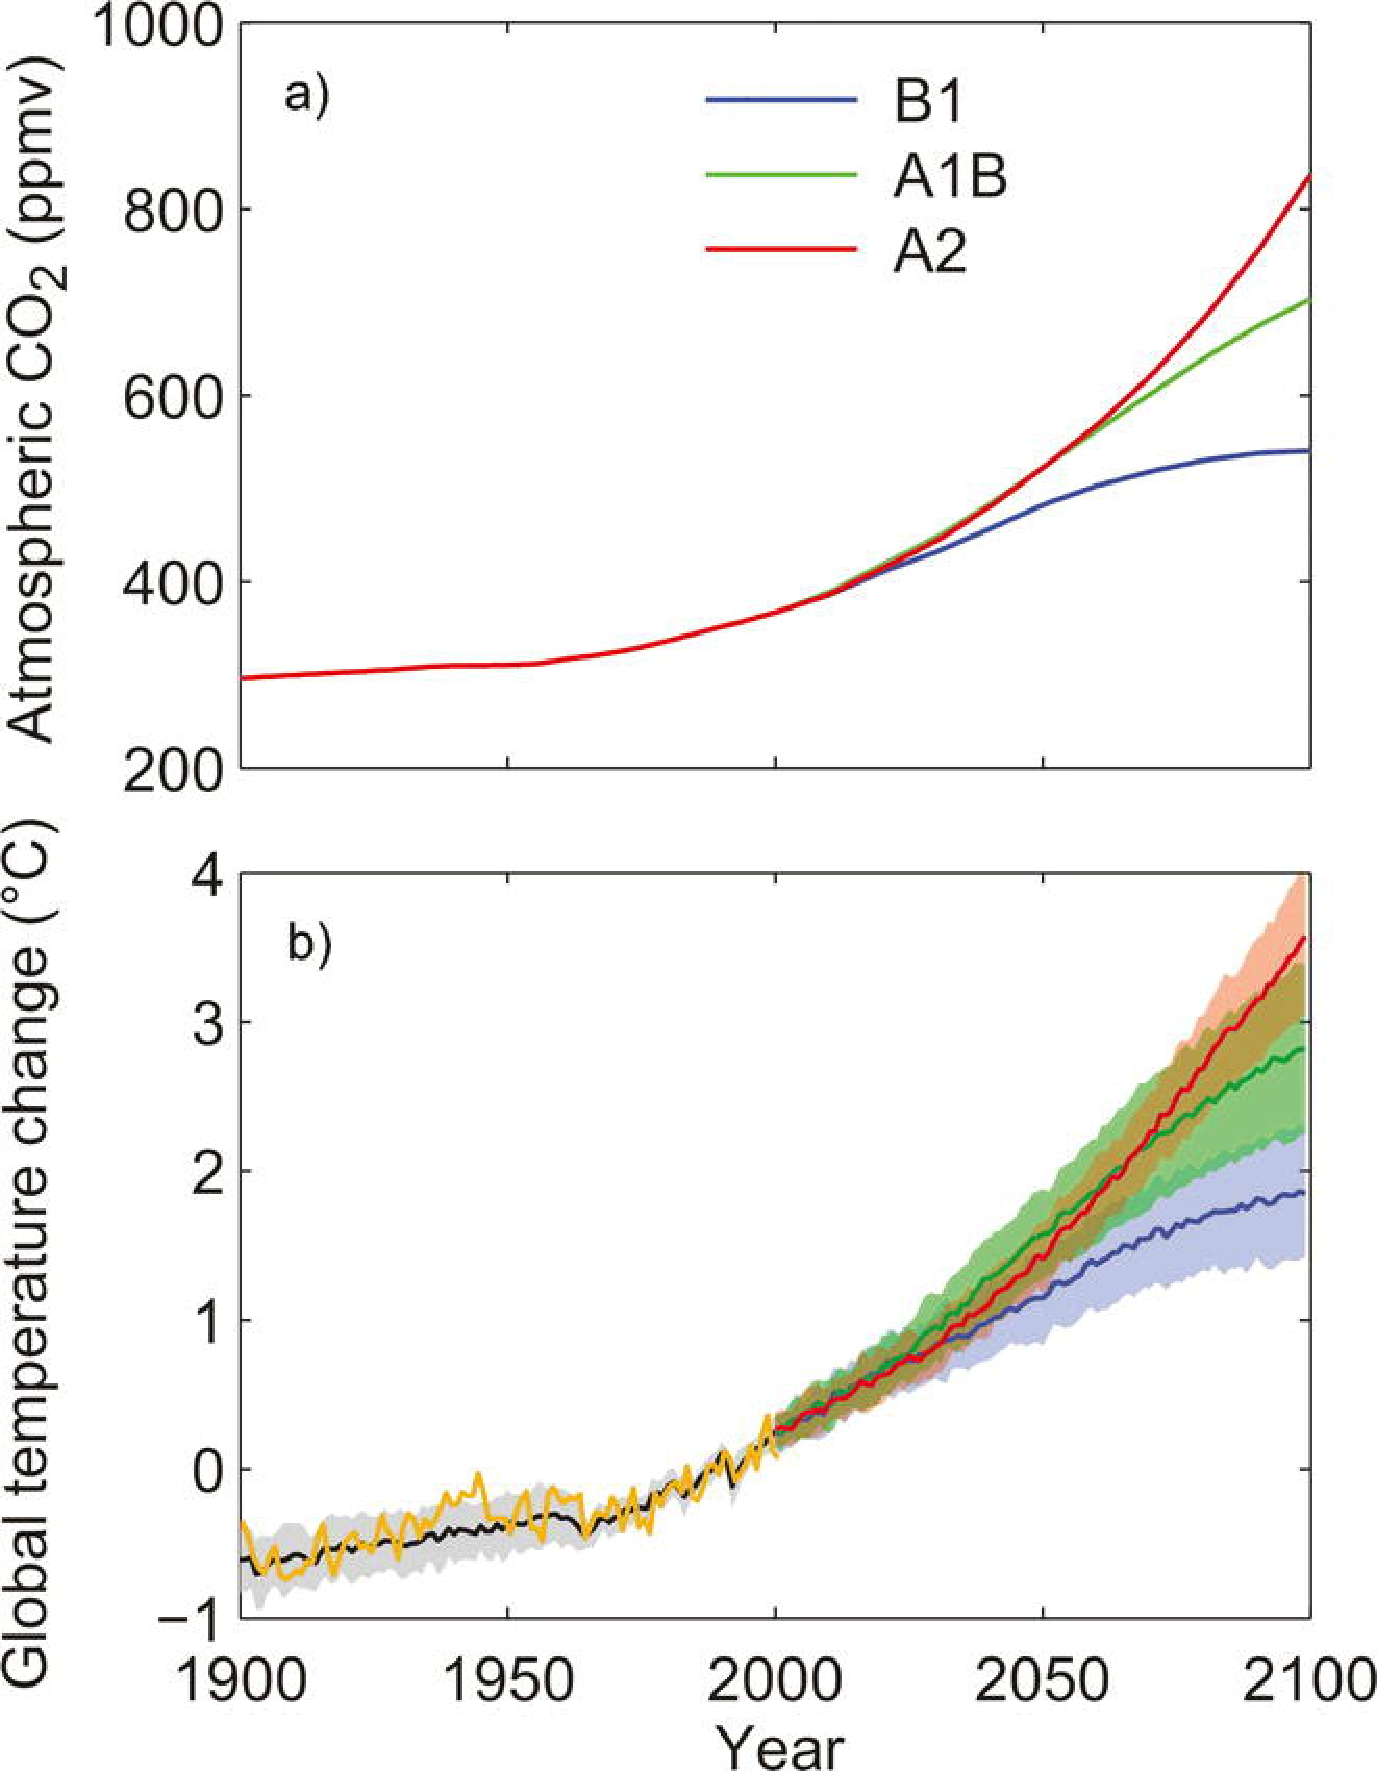
\includegraphics[width=19pc,angle=0]{figure01.pdf}\\
%   \caption{Enter the caption for your figure here.  Repeat as
%     necessary for each of your figures. Figure from \protect\cite{Knutti2008}.}\label{f1}
% \end{figure}

\end{document}

